\chapter{Grundlagen der Signalverarbeitung}
\label{sec:signalFoundations}

Ein \emph{Signal} ist eine Funktion eines Parameters mit numerischen Wertebereich. Die Abbildung zwischen Defintions- und Wertebereich kann, aber muss nicht durch eine Formel definiert sein. So fällt $f(x) = \sin( x )$ genauso unter die Definition eines Signals wie eine Folge numerischer Werte, die durch die Aufnahme eines Messgerätes enstanden sind. Weiterhin kommt dem Wertebereich eine gewissen Bedeutung zu, wie \emph{Zeit} oder \emph{Ort}. Ein typisches Beispiel für ein Signal ist die Spannung, die abhängig von der Zeit von einem Mikrofon erzeugt wird.  Da in dieser Arbeit nur Signale von Bedeutung sind, deren Wertebereich sich auf die Zeit bezieht, konzetrieren sich alle folgenden Bereich auf diesen Bereich- Im Zusammenhang mit Signalen wird der Definitionsbereich auch als \emph{unabhängiger Parameter} und der Wertebereich auch als \emph{abhängiger Parameter} bezeichnet. \cite[S. 11-12]{dspGuide} \cite[S. 22-23]{dspMichigan}

%\emph{ } 
\medskip

 Bei einem zeit-kontinuierlichen Signal $x( \: )$ ist der Wertebereich kontinuierlich, wie in Formel  \ref{eq:time-cont-signal} definiert. Bei einem zeit-diskreten Signal $x[\;]$ ist der Wertebreich diskret, wie in Formel \ref{eq:time-disc-signal} definiert. Abbildung \ref{img:aSignal} zeigt Beispiele für ein zeit-kontinuierliches und ein zeit-diskretes Signal.  So beschreibt beispielsweise $x[17] = s$ den Wert zur Zeit $n = 17$. \glqq Zeit\grqq{} hat in diesem Kontext keine Einheit. Ein Wert wird auch als \emph{Sample} oder \emph{Amplitude} bezeichnet. \cite[S. 22 - 23]{dspMichigan}

 \begin{equation}
x(\;) := \quad \forall t \in \mathbb{R} :\ x(t) = s
\label{eq:time-cont-signal}
\end{equation}


\begin{equation}
x[\;] := \quad  \forall n \in \mathbb{Z} :\ x[n] = s
\label{eq:time-disc-signal}
\end{equation}

\begin{figure}
	\centering
	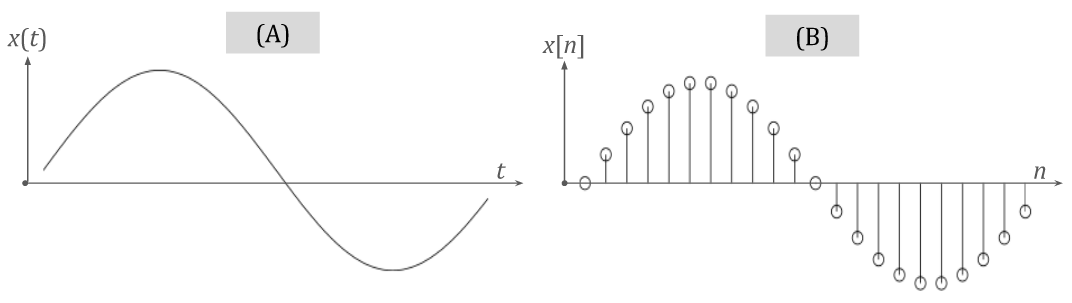
\includegraphics[width=0.7\textwidth]{bilder/aSignal04.png}
	\caption{Ein zeit-kontinuierliches Signal (A) und ein zeit-diskretes Signal (B)}
	\label{img:aSignal}
\end{figure}

Zeit-diskrete Signale werden häufig dadurch gewonnen, dass ein zeit-kontinuierliches Signal in regelmäßigen Intervallen abgetastet wird. Dieser Prozess wird als \emph{Sampling} bezeichnet und durch Formel \ref{eq:sampling} definiert. Der Parameter $T_s$ wird als \emph{Sampling-Interval} bezeichnet. Das Reziproke des Sampling-Intervals heißt \emph{Sampling-Rate} und wird in der Einheit $\frac{1}{\text{s}} = \text{Hz}$, siehe Formel \ref{eq:samplingRate}. Eine Sampling-Rate von $f_s = \SI{44100}{\hertz}$ bedeutete beispielsweise, dass ein Signal 44100 mal pro Sekunde abgetastet wurde.\cite[S. 24]{dspMichigan}

\begin{equation}
x[n] = s(n \cdot T_s) \; , -\infty < n < \infty
\label{eq:sampling}
\end{equation}
	
\begin{equation}
	\text{Samplingrate:} \quad f_s = \frac{1}{T_s} [\text{Hz}]
	\label{eq:samplingRate}
\end{equation}	

Das so genannte \emph{Nyquist-Shannon-Abtasttheorem} nach Formel \ref{eq:shannonTheorem} besagt, dass die Samplingrate mindestens doppelt so hoch sein muss wie die höchste im abgetasteten Signal enthaltene Frequenz. Das bedeutet im Umkehrschluss, dass die höchste im abgetasteten Signal enthaltene Frequenz die Hälfte der Abtastfrequenz entspricht.

\begin{equation}
f_s > 2 \cdot f_{max}
\label{eq:shannonTheorem}
\end{equation}	
	
Da in dieser Arbeit nur zeit-diskrete Signale von Interesse sind, werden ab diesem Punkt die Definitonen für zeit-kontinuierliche Signale ausgelassen. In den beiden Hauptquellen dieser Arbeit, \cite{dspGuide} und \cite{dspMichigan} ist eine Uneinigkeit und Inkonsistent über die symbolische Bezeichung von Signal und Sample festzustellen.  In \cite{dspMichigan} wird die Konvention eingeführt, mit $x[n]$ das gesamte Signal, als auch ein Sample des des Signals zu bezeichnen, was an einigen kritischen Stellen zu unklaren Definitionen führt. In \cite{dspGuide} wird eingeführt, dass das gesamte Signal als $x[\;]$, und ein Sample als $x[n]$ bezeichnet wird. Diese Definition wird im Buch jedoch inkonsistent verwendet und an einigen Stellen $x[n]$ als Bezeichung für das gesamte Signal verwendet.  In dieser Arbeit wird die Konvention eingeführt, mit $x[\;]$ das gesamte Signal, und mit $x[n]$ ein Sample dieses Signals zu bezeichen. Dies führt zwangsweise zur Abwandlung einiger Formeln der beiden Hauptquellen dieses Grundlagenteils, um die Konsistenz beizubehalten.

Der \emph{Support} ist das kleinst mögliche Zeitintervall, der alle Samples enthält, die nicht den Wert 0 haben, wie Formel \ref{eq:support} definiert. 

\begin{equation}
\label{eq:support}
\begin{split}
\text{Sup}(x[\;]) = [sup_s, sup_e] \quad , sup_s, sup_e \in \mathbb{Z} \\,  x[sup_s] \neq 0 \:  \wedge \:  x[sup_e] \neq 0 \: \wedge \: \forall n \
\not\in [sup_s, sup_e] : x[n] = 0
\end{split}
\end{equation}

Die \emph{Dauer} eines Signales ist die Länge des Supportes nach Formel \ref{eq:duration}. In dieser Arbeit herrscht die Konvention, dass die Länge des Signals kurz mit der Variable $N$ abgekürzt wird. Das Signal $x[n] = \cos(n) \: ,0\leq n \leq 3$ hat beispielsweise den Support $[0,3] = \{0,1,2,3\} $ und die Dauer $4$. Ein \emph{unendliches Signal} hat einen unendlichen langen Support, das heißt es gilt Length$(x[\;]) = \infty$. Ein \emph{endliches Signal} hat einen endlichen Support, das heißt Length$(x[\;]) \neq\infty$. Wird in dieser Arbeit der Support nicht explizit angegeben, gilt bei endlichen Signalen als Konvention $Sup(x[\;]) = [0,N-1]$. Unabhängig von der Endlichkeit oder Unendlichkeit des Supportes wird davon ausgegangen, dass sich alle Signale von negativer bis positiver Unendlichkeit erstrecken. Werden also Berechnungen auf Samples eines Signales durchgeführt, die außerhalb seines Supportes liegen, werden diese Samples mit dem Wert 0 angenommen. \cite[S. 24]{dspMichigan}

\begin{equation}
\text{Length}(x[\;]) = sup_e - sup_s + 1 = N
\label{eq:duration}
\end{equation}

Ein Signal gilt als \emph{periodisch}, wenn Formel \ref{eq:periodicity} erfüllt ist. Der Parameter $N$ wird als \text{Periode} von $x[\;]$ bezeichnet. Wenn ein Signal mit $N$ periodisch ist, dann ist es auch mit $2N, 3N, \ldots $ periodisch. Die Grundfrequenz $N_0$ ist das kleinste N, für das Formel \ref{eq:periodicity} erfüllt ist. Abbildung \ref{img:periodicSic} zeigt ein Beispiel für ein nicht-periodisches und ein periodisches Signal. \cite[S. 24]{dspMichigan}

\begin{equation}
\exists N : \forall n \in Sup : x[n+N] = x[n] \rightarrow \text{Periodisch}(x[n]) = true
\label{eq:periodicity}
\end{equation}

\begin{figure}[h]
	\centering
	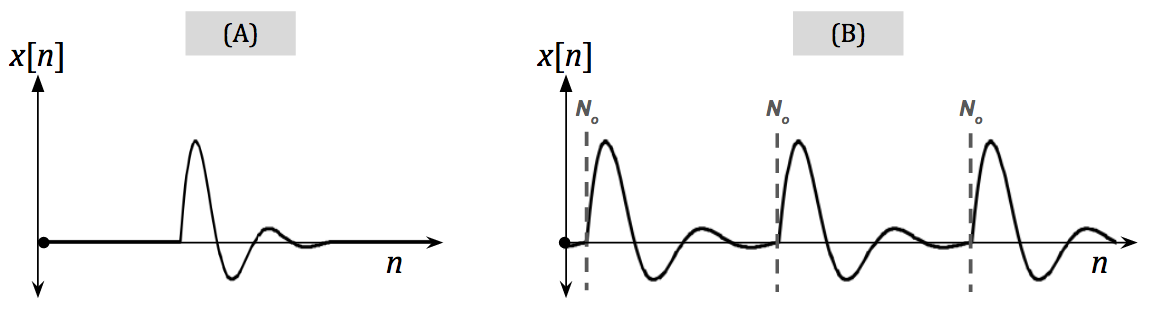
\includegraphics[width=0.8\textwidth]{bilder/periodicSig03.png}
	\caption{Ein nicht-periodisches Signal (A) und ein periodisches Signal (B)}
	\label{img:periodicSic}
\end{figure}

\section{Statistische Merkmale}

Im folgenden wird ein überblick über die häufig verwendete Signaleigenschaften gegeben. Abbildung \ref{img:sigStats} visualisiert die Erläuterungen.

\begin{enumerate}[leftmargin=*]
	
\item Der \textbf{Maximalwert / Minimalwert} beschreibt den höchsten / niedrigsten in  $x[\;]$ enthaltenen Wert nach den Formel \ref{eq:maxAndMin}.

\begin{equation}
\begin{gathered}
 \max(x[\;]) = \max\limits_{n=0\ldots N-1}(x[n]) \\ 
 \min(x[\;])= \min\limits_{n=0\ldots N-1}{n}(x[n])
\end{gathered}
\label{eq:maxAndMin}
\end{equation}

	
\item Der \textbf{Durchschnittswert / Average Value} beschreibt den durchschnittlichen Wert aller Samples von $x[\;]$ nach Formel \ref{eq:avg}. Dieser Durchschnittswert wird über dem Intervall $[n_1, n_2]$  berechnet.

\begin{equation}
\text{AVG}(x[\;]) = \frac{1}{n_2 - n_1 + 1} \sum_{n = n_1}^{n_2} x[n]
\label{eq:avg}
\end{equation}

\item Der \textbf{Mean Squared Value} (\emph{MSV}) beschreibt den quadrierten Durchschnittswert über eine bestimmtes Interval nach Formel \ref{eq:msv}. Er wird auch als \emph{durchschnittliche Energie} oder \emph{average Power} bezeichnet.

\begin{equation}
\text{MSV}(x[\;]) = \frac{1}{n_2 - n_1 + 1} \sum_{n = n_1}^{n_2} x[n]^2
\label{eq:msv}
\end{equation}

\item Das \textbf{Root Mean Square} (\emph{RMS}) ist die Wurzel des Mean Squared Value nach Formel\ref{eq:rms}. Der RMS findet häufiger Anwendung als der MSV, da er besser ins Verhältnis zu den Werten des Signals gesetzt werden kann. Er wird im Deutschen auch als \textbf{Effektivwert} oder \textbf{Durchschnittsleistung} bezeichnet. Da die deutschen Begriffe in einigen Quellen jedoch auch für den MSV verwendet werden, wird an dieser Stelle nur mit den englischen Begriffen gearbeitet.

\begin{equation}
\text{RMS}(x[\;]) = \sqrt{\frac{1}{n_2 - n_1 + 1} \sum_{n = n_1}^{n_2} x[n]^2}
\label{eq:rms}
\end{equation}

\item Die \textbf{Energie / Energy} bezeichnet die \glqq Stärke \grqq{} eines Signals über einen bestimmten Intervall nach Formel \ref{eq:energy}. Sie entspricht dem MSV-Wert multipliziert der Länge des Intervalls. \cite[S. 27-28]{dspMichigan}

\begin{equation}
\text{E}(x[\;]) = \sum_{n = n_1}^{n_2} x[n]^2
\label{eq:energy}
\end{equation}
	
\end{enumerate}	

\begin{figure}[h]
	\centering
	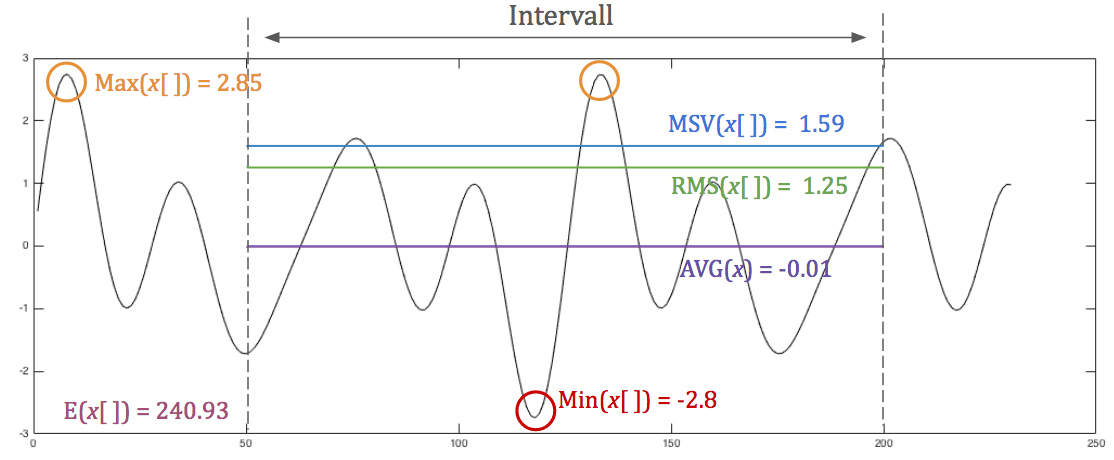
\includegraphics[width=0.7\textwidth]{bilder/sigStats02.png}
	\caption{Statistische Werte eines Signals über das Intervall [50,200]}
	\label{img:sigStats}
\end{figure}

Die Addition und Multiplikation wird bei Signalen komponentenweise durchgeführt, wie Formel \label{eq:addAndMult} definiert.  Abbildung \ref{img:addAndMultSig} visualisiert diese Operationen. 

\begin{equation}
\begin{gathered} 
x_1[\;] + x_2[\;] = y[\;] :=\ \mathop{\forall}_{n = n_1}^{n_2}  :  x_1[n] + x_2[n] = y[n] \\
x_1[\;] \cdot x_2[\;] = y[\;] :=\ \mathop{\forall}_{n = n_1}^{n_2}  :  x_1[n] \cdot x_2[n] = y[n]
\end{gathered}
\label{eq:addAndMult}
\end{equation}

\begin{figure}[h]
	\centering
	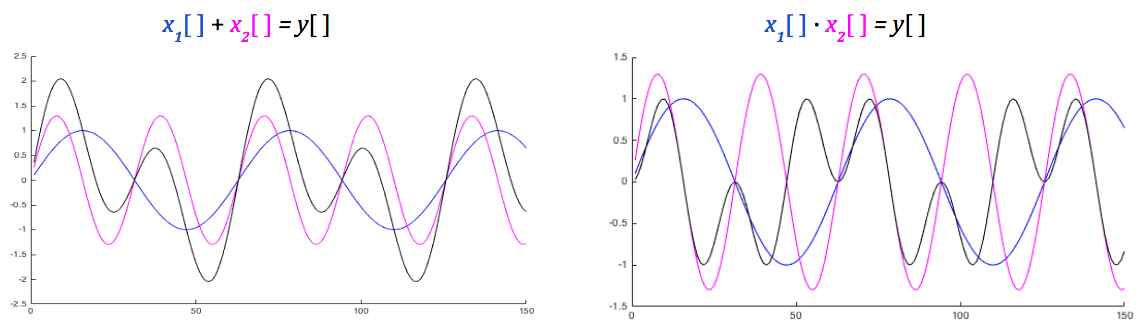
\includegraphics[width=1\textwidth]{bilder/addAndMultSig02.png}
	\caption{Komponentenweise Addition und Mulitplikation zweier Signale}
	\label{img:addAndMultSig}
\end{figure}

\section{Fehlersignale}

Die Addition wird unter anderem für die Modellierung des Einflusses von Störungen benötigt. Angenommen, ein Signal $x[\;]$ wird übertragen, auf dem Übertragungsweg jedoch durch ein anderes Störsignal wie z.B. Rauschen $e[\;]$ überlagert. Dieses Störsignal wird in diesem Zusammenhang auch als \glqq{Fehler-Signal} bezeichnet. Das resultierende Signal $x'[\;]$ wird nach Formel \ref{eq:sigErrorAddition} berechnet. Kennt man sowohl das Eingangssignal $x[\;]$ als auch das Ausgangssignal $x'[\;]$, kann das Störsignal $e[\;]$ nach Formel \ref{eq:calErrorSig} berechnet werden.

\begin{equation}
x'[\;] := \quad \mathop{\forall}_{n = n_1}^{n_2} :\ x'[n] = x[n] + e[n]
\label{eq:sigErrorAddition}
\end{equation}

\begin{equation}
e[\;] := \quad \mathop{\forall}_{n = n_1}^{n_2} :\ e[n] = x'[n] -x[n]
\label{eq:calErrorSig}
\end{equation}

 Errechnet man nun den den MSV- oder RMS-Wert des Störsignales $e[\;]$, gibt das Ergebnis einen Eindrück über die \glqq Stärke \grqq{} des Fehler-Signals. Der MSE-Wert des Fehlers wird in diesem Zusammenhang auch als \emph{Mean Squared Error} (\emph{MSE}) und der RMS-Wert als \emph{Root Mean Squared Error} (\emph{RMSE}) oder einfach als \emph{Fehler} oder \emph{Error} bezeichnet. Formel\ref{eq:mse} und \ref{eq:error} definierten die Berechnungen des MSE und RMSE. Der RMSE hat im Gegensatz zum MSE den Vorteil, dass er besser ins Verhältnis zu den Werten des Fehlersignals gestetzt werden kann. Ein RMSE $= 0$ heisst, dass $x[\;] = x'[\;]$ und somit kein Störsignal vorliegt. Ein RMSE = RMS$(x)$ heisst, dass Eingangs- und Störsignal den selben Effektivwert und somit die selbe \glqq stärke\grqq{} besitzen. Abbildung \ref{img:snrStuff} visualisiert die Berechnung des MSE und RMSE. \cite[S: 28 - 29]{dspMichigan}

\begin{equation}
\text{MSE}(x[\;],x'[\;]) = \frac{1}{n_2 - n_1 + 1} \sum_{n = n_1}^{n_2} (x[n]-x'[n])^2
\label{eq:mse}
\end{equation}

\begin{equation}
\text{RMSE}(x[\;],x'[\;]) = \sqrt{\frac{1}{n_2 - n_1 + 1} \sum_{n = n_1}^{n_2} (x[n]-x'[n])^2}
\label{eq:error}
\end{equation}

Eine weitere Betrachtungsweise bezüglich der Stärke des Rauschens auf das Signal ist, das Eingangssignal ins Verhältnis zum Rauschsignal zu setzen. Formel \ref{eq:snrPre} gibt die Definition. Ein SNR\textsubscript{rel}$(x[\;],e[\;]) = 1$ heißt, dass das Eingangssignal den selben MSV wie das Fehlersignal hat. Meistens ist der MSV des Eingangssignals in der Praxis sehr viel höher als der des Fehler-Signals. Um den Zahlenraum zu begrenzen, wird die Pseudo-Einheit dB verwendet. Formel \ref{eq:snrDb} den so berechneten \emph{Signal-Rausch-Abstand} (\emph{SNR}, englisch Signal-to-Noise-Ratio). Entgegen des MSE weisst ein \emph{niedriger} SNR-Wert auf ein \emph{starkes} Rauschen hin, und ein \emph{hoher} SNR auf ein \emph{schwaches} Rauschen! Abbildung \ref{img:snrStuff} visualisiert die Berechnung des SNR.

%% To do: Gute Quelle suchen!!

\begin{equation}
\text{SNR}_{rel}(x[\;],e[\;]) = \frac{MSV(x[\;])}{MSV(e[\;])}
\label{eq:snrPre}
\end{equation}

\begin{equation}
\text{SNR}(x[\;],e[\;]) = 10 \cdot  \lg \Big(\frac{MSV(x[\;])}{MSV(e[\;])} \Big) \text{ dB}
\label{eq:snrDb}
\end{equation}

\begin{figure}[h]
	\centering
	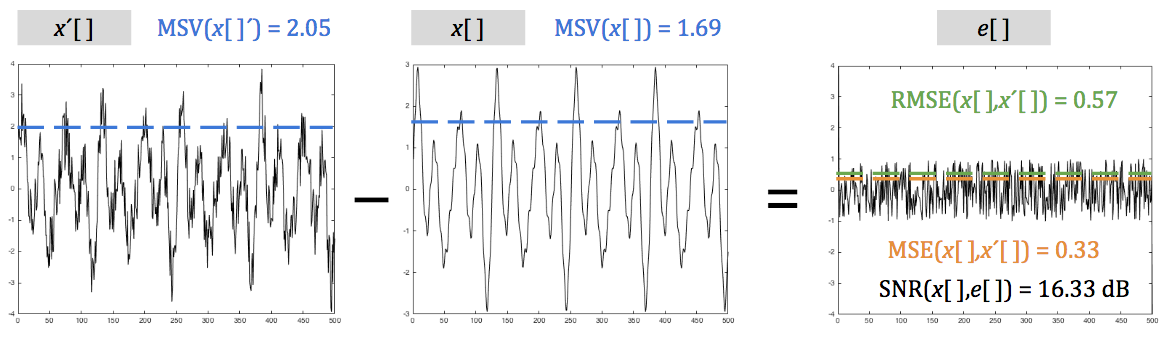
\includegraphics[width=1\textwidth]{bilder/snrStuff04.png}
	\caption{Berechnung des MSE, RMSE und SNR eines von Rauschen gestörten Signals}
	\label{img:snrStuff}
\end{figure}

\section{Korrelation}
\label{sec:correlation}

Die \emph{Korrelation} (engl \emph{Correlation}) zweier Signale $x_1[\;]$ und $x_2[\;]$ wird nach Formel \ref{eq:correlation} als die Summe aller Samples des Produktes der beiden Signale über einen bestimmtes Intervall $[n_1, n_2]$ definiert. Das Ergebnis ist eine Wert $\in \mathbb{R}$ welches die \glqq Ähnlichkeit der beiden Signale\grqq{} kennzeichnet. Ein Positiver Wert weisst auf eine \emph{positive Korrelation} hin, ein negativer Wert auf eine \emph{negative Korrelation}, und ein Wert von $\text{Corr}(x_1[\;],x_2[\;]) = 0$ auf \emph{keine Korrelation}. Aus der größe des Wertes kann die Stärke der Korrelation jedoch nicht direkt interpretiert werden. Bei der \emph{normalisierten Korrelation} Corr$_N(x[\;],y[\;])$ wird daher die Korrelationswert ins Verhältnis zu den Energien der beiden Signale gesetzt, wie in Formel \ref{eq:normCorrelation} definiert. Der Wertebereich der normalisierten Autokorrelation  ist $-1 \leq \text{Corr}_N(x[\;],y[\;]) \leq +1$. Daraus ergeben sich die in Formel \ref{eq:correlationProps} definierten Zusammenhänge. Ein Wert von $ \text{Corr}_N(x[\;],y[\;]) = 1$ wird auch als \emph{perfekte Korrelation} bezeichnet, ein Wert von  $ \text{Corr}_N(x[\;],y[\;]) = -1$ als \emph{anti-perfekte Korrelation} \cite[S. 46 - 47]{dspMichigan} Abbildung \ref{img:corrSigsComp} visualisiert die normalisierte Korrelation eines Signales $x[\;]$ mit den Signalen $y[\;]$.

\begin{equation}
\text{Corr}(x[\;],y[\;]) = \sum_{n=n_1}^{n_2} x[n] \cdot y[n]
\label{eq:correlation}
\end{equation}

\begin{equation}
\text{Corr}_N(x[\;],y[\;]) = \frac{\text{Corr}(x[\;],y[\;])}{\sqrt{\text{E}(x[\;]) \cdot \text{E}(y[\;])}}
\label{eq:normCorrelation}
\end{equation}

\begin{equation}
\text{Corr}_N(x[\;],y[\;]) = 
\begin{cases}
1  \quad \rightarrow  x[\;] = y[\;] \\
-1 \; \rightarrow x[\;] = -y[\;]
\end{cases}
\label{eq:correlationProps}
\end{equation}

\begin{figure}[h]
	\centering
	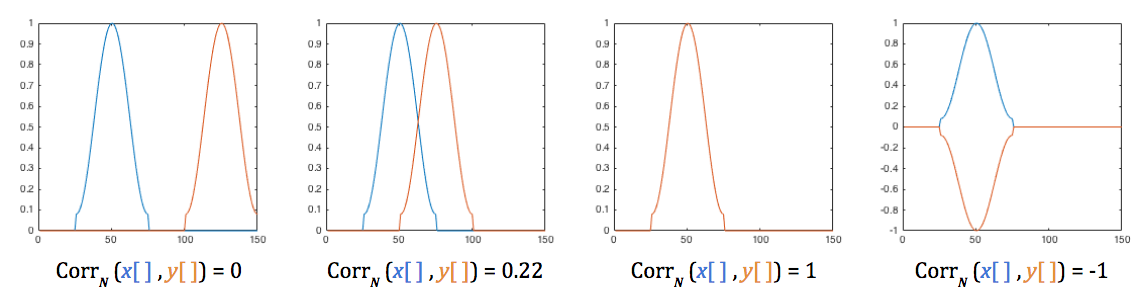
\includegraphics[width=1\textwidth]{bilder/corrSigsComp02.png}
	\caption{Correlation der Signale $x[n]$ und $y[n]$}
	\label{img:corrSigsComp}
\end{figure}

Die Korrelation und die normalisierte Korrelation werden aufgrund ihrer Eigenschaften verwendet, um ein Signal $x[\;]$ in einem Signal $y[\;]$ zu detektieren. Häufig ist das Ziel, ein von einem Rauschen $e[\;]$ überlagerten Signal $x[\;]+e[\;] = y[\;]$ auf das Vorhandensein des erwarteten Signales $x[\;]$ hin zu überprüfen. Wie in Abbildung \ref{img:corrSigsComp} zu sehen ist, ist der Korrelationswert jedoch von der Verzögerung des Signals abhängig. Daher wird in der $Cross-Correlation$ das Signal $y[\;]$ mit einer verzögerten Varianten des Signals $x[\;]$ korreliert, wie in Formel \ref{eq:XCorr} definiert. Der parameter $k$ wird als \emph{Lag} bezeichnet und gibt die Verzögerung an. 

\begin{equation}
\text{X-Corr}_k(x[\;],y[\;]) = \sum_{n=-\infty}^{\infty} x[n-k] \cdot y[n]
\label{eq:XCorr}
\end{equation}

Im Prozess der so genannten \emph{Running Correlation} nutzt man die Cross-Correlation mit den Lags $k = 0 \cdots k_{max}$ zur Erstellung des \emph{Korrelationssignals} $r[\;]$, wie in Gleichung \ref{eq:runningCorrelation} definiert. Das Signal $r[\;]$ gibt Auskunft, zu welchen Verzögerungswerten $k$ die größten Ähnlichkeiten zwischen $x$ und $y$ gefunden wurden. 

\begin{equation}
r[\;] := \quad \mathop{\forall}_{k = 0}^{k_{max}} :\ r[k] = \text{X-Corr}_k(x[\;],y[\;])
\label{eq:runningCorrelation}
\end{equation}

Abbildung \ref{img:slidingCorrelation} zeigt ein Beispiel für die Erzeugung von $r[\;]$ mit der Sliding Correlation. (A) zeigt das zu detektierende Signal $x[\;]$ und (B) das Signal $y[\;]$. (C) zeigt das Korrelationssignal $r[\;]$ mit den Lags $k = 0, \ldots ,1150$ . \cite[S. 47 - 48]{dspMichigan}

\begin{figure}[h]
	\centering
	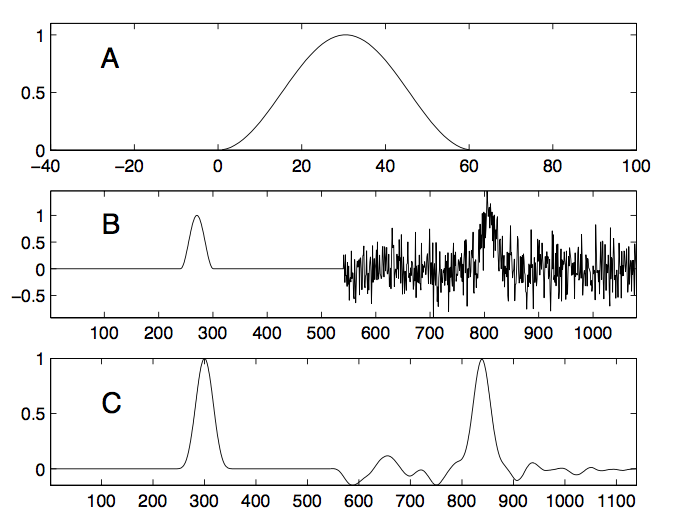
\includegraphics[width=0.5\textwidth]{bilder/slidingCorrelation.png}
	\caption{Beispiel einer Running Correlation}
	\label{img:slidingCorrelation}
\end{figure}


\section{Diskrete Fourier-Transformation}

Die \emph{Fourier-Transformation} ist eine Familie von Transformationen, mit deren Hilfe Signale aus dem Zeit-Bereich in den Frequenz-Bereich transformiert werden. Das heißt, dass der unabhängige Parameter nach der Transformation nicht mehr die Zeit, sondern die Frequenz beschreibt. 

Die konkrete Berechnung der Transformation ist abhängig von den Eigenschaften des Signales. Die Variante, die die meiste Anwendung in der digitalen Signalverarbeitung findet, ist die \emph{Diskrete Fourier-Transformation} (kurz \textbf{DFT} ). Sie transformiert \emph{zeit-diskrete, periodische, unendliche} Signale (siehe Formel \ref{eq:time-disc-signal} und \ref{eq:periodicity}) in den Frequenz-Bereich. Es exisitert sowohl eine reelle als auch eine complexe Variante der DFT. Die reelle Variante wird mit Hilfe reeller Zahlen, und die komplexe mit Hilfe komplexer Zahlen berechnet. An dieser Stelle werden beide Variante vorgestellt: Die komplexe, da der effizienteste Algorithmus zur Berechnung der DFT, die \emph{Fast-Fourier-Transformation} (\textbf{FFT}) auf ihr beruht, und die reelle, da sie das Verständnis der komplexen vereinfacht.\cite[S. 142 - 146]{dspGuide}

\subsection{Reelle DFT}
\label{sec:realDFT}

Jedes zeitdiskretes, periodisches Signal $x[\;]$ kann erzeugt werden, indem eine endliche Anzahl von Sinus- und Cosinus-Signalen geeigneter Frequenz und Amplitude aufaddiert werden. Der Umkehrschluss ist, dass sich jedes Signal in eine Menge von Sinus- und Cosinus-Signalen zerlegen lässt, ohne das Information für das Signal $x[\;]$ verloren geht. Diese Zerlegung des Signals $x[\;]$ wird als \emph{Dekomposition} bezeichnet, die Kombination der Sinus- und Cosinus-Siganel zu $x[\;]$ als \emph{Synthese}. Genauer gesagt werden für ein Signal $x[\;]$ mit Length$(x[\;]) = N$ höchstens $\frac{N}{2}+1$ Sinus- und $\frac{N}{2}+1$ Cosinus-Wellen benötigt, also insgesamt $N+2$ Signale. Gleichung \ref{eq:fftIntroduction} fasst diese Aussage zusammen. \cite[S. 144 - 147 ]{dspGuide}

\begin{equation}
\label{eq:fftIntroduction}
\begin{split}
x[\;] := \quad \mathop{\forall}_{n = 0}^{N-1} :\ x[n] =  A[0]\cos_{f_0}[n] + \ldots + A[N/2]\cos_{f_{N/2}}[n]  \\ + B[0]\sin_{f_{N/2}}[n] + \ldots + B[N/2] \sin_{f_{N/2}}[n]
\end{split}
\end{equation}


Die Cosinus- und Sinus-Schwingungen, die in Gleichung \ref{eq:fftIntroduction} verwendet werden, werden in Gleichung \ref{eq:cosine} definiert. Die Faktoren $A[\;],B[\;]$ geben die Amplitude der entsprechenden Cosinus/Sinus-Schwingung an, der Fatkor $f$ die Frequenz der Schwingung (Perioden pro Sekunde), und $f_s$ die Sampling-Rate (Siehe Gleichung \ref{eq:samplingRate}). \cite[S. 62]{dspMichigan} \cite[S. 150]{dspGuide} Abbildung \ref{img:aSimpleCosine} zeigt ein Beispiel für die Cosinus-Schwingung $[A_f=2] \cdot cos_{f=\SI{4}{\hertz}}[\;]$.

\begin{equation}
\label{eq:cosine}
\begin{gathered}
\cos_{f}[n]  = \cos(2\pi f \frac{n}{f_s}) \\
\sin_{f}[n]  = \sin(2\pi f \frac{n}{f_s})
\end{gathered}
\end{equation}

\begin{figure}[h]
	\centering
	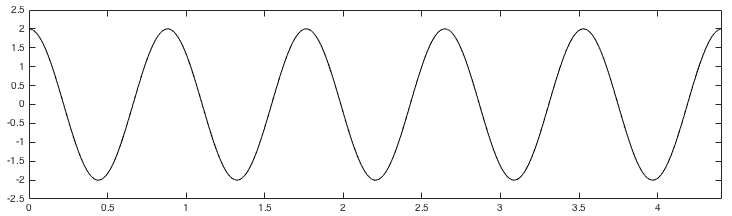
\includegraphics[width=0.7\textwidth]{bilder/aSimpleCosine.png}
	\caption{$\SI{1}{\second} = 44100 $ Samples der Cosinus-Schwingung $[A = 2] \cdot cos_{f=\SI{4}{\hertz}}[\;] =  2 \cdot \cos(2\pi 4 \frac{n}{f_s})$ bei einer Sampling-Rate von $f_s = \SI{44100}{\hertz} $}
	\label{img:aSimpleCosine}
\end{figure}

Abbildung \ref{img:fftExample02} zeigt ein Beispiel für die Synthese eines Signal $x[\;]$ mit $N = 200$ Samples mit einer Samlingrate von $f_s = \SI{100}{\hertz}$. Es werden theoretisch $\frac{N}{2} + 1 = 101$ Cosinus und $101$ Sinus-Signale für die Synthese benötigt, da aber nur 4 Signale eine Amplitude $> 0$ haben, werden auch nur diese Signale gezeigt. Die Frage ist: Angenommen, man kennt nur das Signal $x[\;]$, wie errechnet man daraus die die Amplituden $A[\;], B[\;]$ und Frequenzen $f$ der Cosinus- und Sinus-Signale? Anders gesagt: Wie berechnet man die Dekomposition?

\begin{figure}[h]
	\centering
	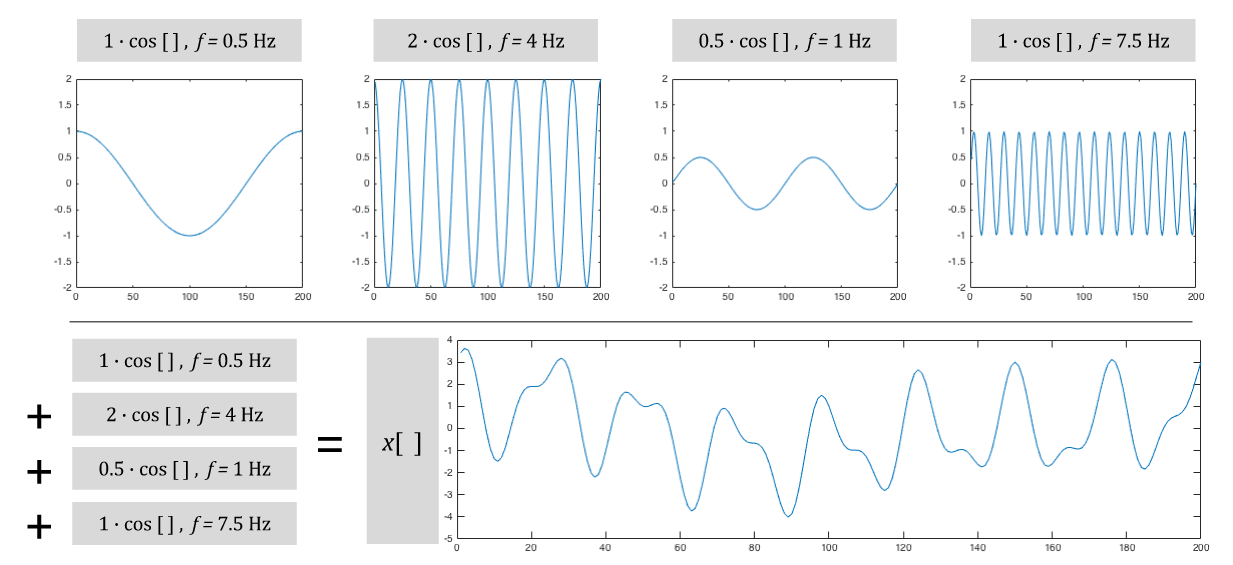
\includegraphics[width=1\textwidth]{bilder/fftExp05.png}
	\caption{Synthetisierung eines Signals $x[\;]$ aus vier Cosinus-Funktionen, mit Length$(x[\;]) = 200$ und $f_s = \SI{100}{\hertz}$}
	\label{img:fftExample02}
\end{figure}

Das Problem lässt sich auf die Berechnung der Amplituden $A[\;],B[\; ]$ beschränken, in dem man den Fakt, dass höchstens $\frac{2}{N} + 1$ Cosinus- und $\frac{2}{N} + 1$ Sinus-Signale für die Synthese benötigt werden, in Verbindung mit dem Nyquist-Shannon-Abtasttheorem (Gleichung \ref{eq:shannonTheorem}) bringt. Die niedrigst mögliche Frequenz, die im Signal $x[\;]$ enthalten sein kann, ist $f_0 = \SI{0}{\hertz}$, und die höchst mögliche Frequenz $f_{max} = \frac{f_s}{2}$, womit die Frequenzen der Signale $\cos_{f_0 = 0}[\;] , \cos_{f_{max} = f_s/2}[\;],\sin_{f_0 = 0}[\;], \sin_{f_{max} = f_s/2}[\;]$ bereits feststehen. Die restlichen $\frac{2}{N} - 1$ Cosinus-Signale teilen sich gleichmäßig auf diesen Frequenzraum auf, entsprechendes gilt für die Sinus-Signale. Die Frequenz der insgesamt $N+2$ Cosinus/Sinus-Signale ergibt sich somit direkt als Funktion der Samplingrate und der Länge des Signals $x[\;]$. Gleichung \ref{eq:baseFunctions} fasst diesen Zusammenhang zusammen. Die dort beschriebenen Funktionen $\cos_k[\;]$ und $\sin_k[\;]$werden als \emph{Basisfunktionen} bezeichnet. Aus dem  Index $k = 0 ,\ldots, \frac{N}{2}$ lässt sich die Frequenz der jeweiligen Basisfunktion nach Gleichung \ref{eq:baseToFreq} berechnen.\cite[140 - 151, S.]{dspGuide}  In Bezug auf das Beispiel aus Abbildung \ref{img:fftExample02} ergeben sich die Indexe $[\cos_{f=\SI{0.5}{\hertz}}[\;] = \cos_1[\;]]$, $[\cos_{f=\SI{4}{\hertz}}[\;] = \cos_8[\;]]$, $[\sin_{f=\SI{1}{\hertz}}[\;] = \sin_2[\;]]$ und $[\sin_{f=\SI{7.5}{\hertz}}[\;] = \sin_{15}[\;]]$

\begin{equation}
\label{eq:baseFunctions}
\begin{split}
\cos_k[\;] := \quad \mathop{\forall}_{n = 0}^{N-1} :\ \cos_k[n] = \cos(2\pi k \frac{n}{N}) \\
\sin_k[\;] := \quad \mathop{\forall}_{n = 0}^{N-1} :\ \sin_k[n] = \sin(2\pi k \frac{n}{N}) \\
N = \text{Length} (x[\;] )
\end{split}
\end{equation} 

\begin{equation}
\label{eq:baseToFreq}
f = k\frac{f_s}{N} 
\end{equation} 

Das Problem der Dekomposition wird so auf die Suche der Amplituden-Koeffizienten $A[k], B[k]$ beschränkt, die zu den jeweiligen Basisfunktionen $\cos_k[\;]$ und $\sin_k[\;]$ gehören. Die Frage ist, vereinfacht formuliert, wie \glqq stark\grqq{} jede der Basisfunktionen $\cos_0[\;], \ldots ,\cos_{N/2}[\;]$ und $\sin_0[\;] ,\ldots ,\sin_{N/2}[\;]$ in $x[\;]$ enthalten ist.  Die Antwort darauf ist die in Kapitel \ref{sec:correlation} vorgestellte Korrelation. Der Korrelationswert einer Cosinus-Basisfunktion mit Eingangssignal Corr$(x[\;],\cos_k[\;]) = \sum_{n=0}^{N-1} \cdot x[n]cos_k[n]$ gibt somit eine Aussage darüber, wie stark die entsprechende Cosinus-Schwingungen zur Syntehse von $x[\;]$ beiträgt. Ein Wert von $0$ spricht für keinen Beitrag, ein hoher oder niedriger Wert für eine positiven oder negativen Beitrag. \cite[S. 157 - 158]{dspGuide}

Dieses Vorgehen lässt sich sogenannten \emph{forward DFT} nach Formel \ref{eq:forwardDFT} verallgemeinern, kurz als \textbf{DFT} bezeichnet. Das Ergebnis sind die Koeffizienten $\bar{A}[\;] = \bar{A}[0]\ldots \bar{A}[N/2]$ und $\bar{B}[\;] = \bar{B}[0] \ldots \bar{B}[N/2]$. Die Koeffizienten werden gemeinsam als der \emph{Frequenz-Bereich} in \emph{kartesischer Notation} $X[\;]$ bezeichnet. Das $X[\;]$ hat im Zusammenhang mit der reellen DFT einen rein symbolisch bezeichnenden Charakter und wird erst im Zusammenhang mit der \emph{komplexen DFT} in Kapitel \ref{sec:comDFT} zu einem Signal.  \cite[S. 158]{dspGuide}

\begin{equation}
\text{DFT}\{x[\;]\} = X[\;] :=
\begin{dcases}
\bar{A}[\;]  := \mathop{\forall}_{k = 0}^{N/2} :\ \bar{A}[k] = \sum_{n=0}^{N-1}x[n] \cos(2\pi k \frac{n}{N}) \\
 \bar{B}[\;] := \mathop{\forall}_{k = 0}^{N/2} :\ \bar{B}[k] = \sum_{n=0}^{N-1}x[n] \sin(2\pi k \frac{n}{N}) 
\end{dcases}
\label{eq:forwardDFT}
\end{equation}

In Bezug auf das Beispiel aus Abbildung \ref{img:fftExample02} ergeben sich bei Anwendung von Formel \ref{eq:forwardDFT} auf das Signal $x[n]$ die Koeffizienten $[ \bar{A}_{f=\SI{0.5}{\hertz}} = \bar{A}[1] = 100 ]$ , $[  \bar{A}_{f=\SI{4}{\hertz}} = \bar{A}[8] = 200 ]$, $[ \bar{B}_{f=\SI{1}{\hertz}} = \bar{B}[2] = 50 ]$ und $[ \bar{B}_{f=\SI{7.5}{\hertz}} = \bar{B}[15] = 100 ]$. Um die eigentlichen Koeffizienten $A[1] = 1, A[8] = 2, B[2] = 0.5$ und $B[[15] = 1$ zu erhalten, muss die Umrechnungsvorschrift nach den Formel \ref{eq:AConversion} und \ref{eq:BConversion} angewandt werden. Dieser Transformationsschritt $\bar{A}[\;] \longmapsto  A[\;]$ und $\bar{B}[\;] \longmapsto  B[\;]$ ist ein \emph{Extra-Schritt}, den jeder reelle DFT nach sich zieht. \cite[S. 152 - 153]{dspGuide}

\begin{equation}
A[\;] := \quad \mathop{\forall}_{k = 0}^{N/2} :\ A[k] = 
\begin{dcases}
\frac{\bar{A}[k]}{N} \quad, \text{falls } k = 0 \vee k = N/2\\
\frac{\bar{A}[k]}{N/2} \quad ,\text{sonst} \\
\end{dcases}
\label{eq:AConversion}
\end{equation}

\begin{equation}
B[\;] := \quad \mathop{\forall}_{k = 0}^{N/2} :\
B[k]= \frac{B_k}{N/2}
\label{eq:BConversion}
\end{equation}

Gleichung \ref{eq:inverseDFT} definiert die Synthese des Signals $x[\;]$ aus den Basis-Funktionen mit Hilfe der Koeffizienten $A[\;]$ und $B[\;]$. Die Formel wird auch als \emph{inverse DFT} (\textbf{iDFT}) bezeichnet. \cite[S. 152 - 153]{dspGuide}

\begin{equation}
\text{DFT}\{X[\;]\} = x[\;]
:= \quad \mathop{\forall}_{n = 0}^{N-1} :\ x[n] = \sum_{k = 0}^{N/2} A[k]\cos(2\pi k \frac{n}{N}) + \sum_{k = 0}^{N/2}B[k]\sin(2\pi k \frac{n}{N}) \\
\label{eq:inverseDFT}
\end{equation}

Abbildung \ref{img:dtOverview} gibt einen Überblick über den Zusammenhang $x[\;]$ und $X[\;]$. Da mit steigender Länge von $x[\;]$ die Anzahl an Basis-Funktionen im Frequenzbereich $X[\;]$ steigt, wird die Auflösung des Frequenz-Bereiches umso höher, je länger $x[\;]$ gewählt wird. Im Gegenzug sinkt die Auflösung in Bezug auf den Zeit-Bereich: Der Frequenz-Bereich trifft keine Aussage darüber \emph{wann} etwas passiert, sondern nur \emph{welche Frequenzen} daran beteiligt sind.\cite[S. 170]{dspGuide}

\begin{figure}[h]
	\centering
	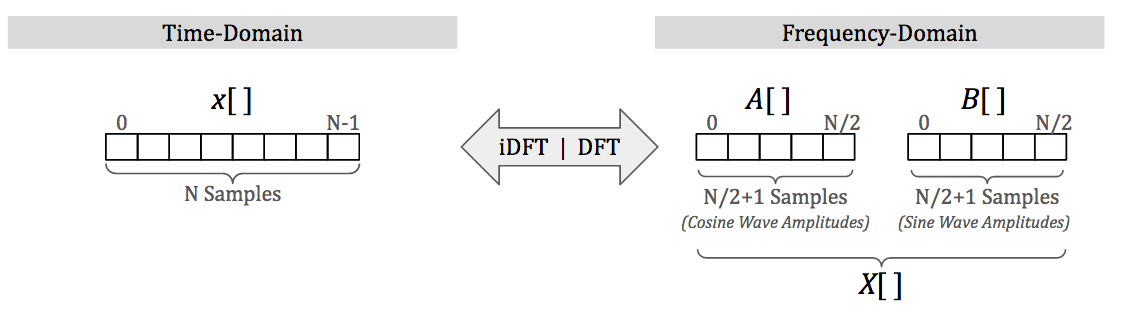
\includegraphics[width=1\textwidth]{bilder/dftOverview04.png}
	\caption{Überblick über die DFT und die inverse DFT}
	\label{img:dtOverview}
\end{figure}

Aus Formel \ref{eq:inverseDFT} geht hervor, dass bei der Synthese jeweils ein Cosinus-Signal und ein Sinus-Signal der selben Frequenz addiert wird. Diese Addition erzeugt einen sogenannten \emph{Sinusoiden}, eine Cosinuswelle mit der Amplitude $M$ der Phasenverschiebung $\phi$ nach Formel \ref{eq:sinusoid}.\cite[S. 162]{dspGuide}

\begin{equation}
\begin{split}
A \cos(x) + B \sin(x) = M \cos(x + \phi) \\
,M = \sqrt{A^2 + B^2} \quad, \phi = arctan(B/A)
\end{split}
\label{eq:sinusoid}
\end{equation}

Auf Basis von Formel \ref{eq:sinusoid} lässt sich der gesamte Frequenz-Bereich in kartesischer Notation als Menge von Sinusoiden-Schwingungen mit den Magnituden $M[\;] = M[0] \ldots M[N/2]$ und den Phasenverschiebungen $\phi[\;] = \phi[0] \ldots \phi[N/2]$ ausdrücken. Formel \ref{eq:rectToPolar} definierte diese Transformation des Frequenz-Bereichs von kartesischer Notation in die \emph{polare Notation}. Formel \label{eq:polarToRect} definiert die dazu inverse Transformation. \cite[S. 162]{dspGuide} Abbildung \ref{img:polarToRect02} zeigt den Frequenzbereich in polarer Notation für das Beispiel aus  Abbildung \ref{img:fftExample02}.

\begin{equation}
(A[\;], B[\;]) \longmapsto (M[\;], \phi[\;])  = 
\begin{dcases}
M[\;] := \mathop{\forall}_{k = 0}^{N/2} :\ M[k] = \sqrt{(A[k]^2 + B[k]^2 ) }   \\
 \phi[\;]  := \mathop{\forall}_{k = 0}^{N/2} :\ \phi[k]= \arctan{(B[k] / A[k]) }
\end{dcases}
\label{eq:rectToPolar}
\end{equation}

\begin{equation}
(M[\;], \phi[\;]) \longmapsto (A[\;], B[\;])  =
\begin{dcases}
A[\;]  := \mathop{\forall}_{k = 0}^{N/2} :\ A_k= M_k \cdot \cos(\phi_k) \\
B[\;]  := \mathop{\forall}_{k = 0}^{N/2} :\ B_k = M_k \cdot \sin(\phi_k)
\end{dcases}
\label{eq:polarToRect}
\end{equation}

Die kartesische Notation wird verwendet, um die DFT und die inverse DFT zu berechnen. Die polare Notation hat den Vorteil, dass vor allem die Magnituden $M[\;]$ für den Menschen leichter zu interpretieren sind. Die Magnituden $M[\;]k$ sind Audioingenieuren als \emph{Spectrum} bekannt und werden in dieser Arbeit auch als solches bezeichnet. Die Phasen-Informationen $\phi[\;]$ hingegen haben für das menschliche Gehör kaum Einfluss und wird daher, zumindest bei der Betrachtung durch den Menschen, kaum Einfluss. \cite[Signals and transforms, S. 10 ]{ricardo_ceps} Die Transformation in die polare Notation wird deshalb vor allem dann Angewandt, wenn der Mensch den Frequenz-Bereich interpretieren soll. \cite[S. 164]{dspGuide}

\begin{figure}[h]
	\centering
	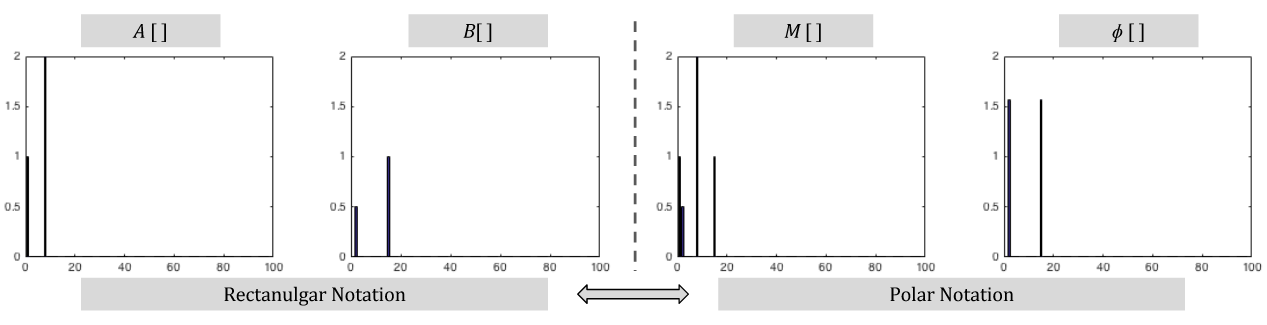
\includegraphics[width=1\textwidth]{bilder/rectToPolar03.png}
	\caption{Frequenz-Bereich des Beispiels aus Abbildung \ref{img:fftExample02}}
	\label{img:polarToRect02}
\end{figure}

Ein Schlussbemerkung: In der Einleitung dieses Kapitels wurde erwähnt, dass die DFT \emph{zeit-diskrete, periodische, unendliche} Signale transformiert, während in der hier vorgestellten Erläuterung das Signal sowohl als endlich angenommen, als auch keine Aussage über die Periodizität gemacht wurde. Bei der DFT wird davon ausgegangen, dass das Signal \emph{außerhalb} des Supportes von $x$ unendlich oft wiederholt wird, um die Vorraussetzungen zu erfüllen. Dabei handelt es sich jedoch um einen \glqq matehmatischen Trick \grqq{} der nur in Ausnahmefällen Einfluss auf den Frequenz-Bereich hat. Diese Ausnahmefälle tangieren diese Arbeit jedoch nicht, weshalb sie an dieser Stelle nicht weiter erläutert werden.\cite[S. 145]{dspGuide}

\subsection{Komplexe DFT}
\label{sec:comDFT}

Gleichwohl die in Kapitel \ref{sec:realDFT} vorgestellte \emph{reelle DFT} hilft beim Verständnis des Frequenz-Bereiches hilft, ist die Berrechnung der DFT nach Formel \ref{eq:forwardDFT} Rechnerisch zu ineffizient, um in Echtzeit durchgeführt zu werden. Der am weitesten verbreitete Algorithmus zur Berechnung des Frequenz-Bereiches, die \emph{Fast Fouerier-Transformation} erlaubt hingegen die Berechnung der DFT in Echtzeit. Da die FFT auf der \emph{complexen} Variante der DFT basiert, wird sie an dieser Stelle vorgestellt. \cite[S. 225]{dspGuide}

Die Basis der komplexen DFT ist die \emph{Eulerformel}, definiert in Formel \ref{eq:eulersRelation}. Sie erlaubt die Darstellung des Funktions-Werte einer Cosinus-Welle und einer Sinus-Welle der selben Frequenz und Amplitude als den Real/Imaginärteil eines komplexen Exponenten der Eulerschen Zahl $e$. Gleichung \ref{eq:eulersRelationDetailed} zeigt, dass die Isolierung des Real/Imaginärteil von $e^{ix}$ Zugriff auf Funktionswert der entsprechenden Cosinus/Sinuswelle erlaubt. Außerdem werden die Funktionen $|e^{ix}|$ und $\phi(e^{ix})$ definiert. Abbildung \ref{img:eulersRelation} visualisiert diese Zusammenhänge. Auf einen Beweis der Eulergleichung wird an dieser Stelle aus Platzgründen verzichtet. \cite[S. 569]{dspGuide}

\begin{equation}
e^{ix} = \cos(x) + i\sin(x)
\label{eq:eulersRelation}
\end{equation}

\begin{equation}
\begin{gathered}
\Re(e^{ix}) = \cos(x) \\
\Im(e^{ix}) = \sin(x)  \\
|e^{ix}| = \sqrt{\cos(x)^2 + \sin(x)^2} \\
\phi (e^{ix}|) = \arctan (\frac{\sin(x)}{\cos(x)})
\end{gathered}
\label{eq:eulersRelationDetailed}
\end{equation}

\begin{figure}[h]
	\centering
	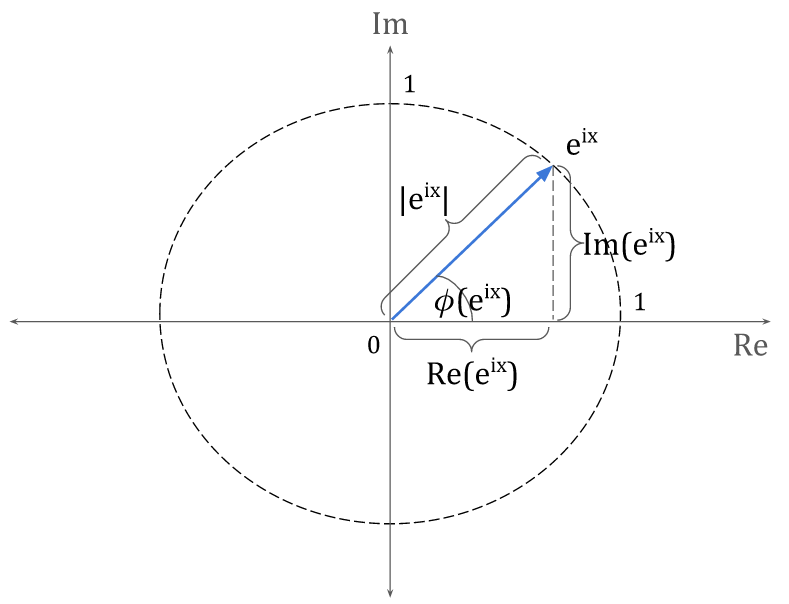
\includegraphics[width=0.5\textwidth]{bilder/eulersRelation02.png}
	\caption{Visualisierung der Eulergleichung}
	\label{img:eulersRelation}
\end{figure}

Dementsprechend lassen sich die Basisfunktionen aus Gleichung \ref{eq:baseFunctions} ebenfalls durch den Real/Imaginärteil der von $e^{ix}$ nach Gleichung \ref{eq:complexBaseFunktion} definieren. Sie werden als die \emph{komplexe Basisfunktionen} bezeichnet. Die Frequenz der jeweiligen Basisfunktion wird, wie in Formel \ref{eq:baseToFreq} definiert, durch  $f = k\frac{f_s}{N}$ errechnet. 

\begin{equation}
\begin{gathered}
\cos_k[\;] := \quad \mathop{\forall}_{n = 0}^{N-1} :\  \Re(e^{i\cdot 2\pi k \frac{n}{N}}) = \cos_k[n] = \cos(2\pi k \frac{n}{N}) \\
\sin_k[\;] := \quad \mathop{\forall}_{n = 0}^{N-1} :\ \Im(e^{i\cdot 2\pi k \frac{n}{N}}) = \sin_k[n] = \sin(2\pi k \frac{n}{N})
\end{gathered}
\label{eq:complexBaseFunktion}
\end{equation}

Auf Basis dieses Zusammenhanges wird die \emph{komplexe DFT} in \emph{kartesischer Notation} nach Formel \ref{eq:complexDFTrectanulgar} definiert, das heißt die Transformation vom Zeit-Bereich in den Frequenzbereich mit Hilfe komplexer Zahlen. Formel \ref{eq:complexDFTpolar} definiert die komplexe DFT in der kompakteren, \emph{polaren Notation}. \cite[S. 570]{dspGuide}

\begin{equation}
\label{eq:complexDFTrectanulgar}
\text{DFT}\{x[\;]\} = X[\;]  := \quad \mathop{\forall}_{k = 0}^{N-1} :\ X[k] = \frac{1}{N} \sum_{n = 0}^{N-1}  x[n] \cdot (\cos (2\pi k \frac{n}{N}) -i \sin (2 \pi k \frac{n}{N}) )
\end{equation}

\begin{equation}
\label{eq:complexDFTpolar}
\text{DFT}\{x[\;]\} = X[\;]  := \quad \mathop{\forall}_{k = 0}^{N-1} :\ X[k] =  \frac{1}{N} \sum_{n = 0}^{N-1}  x[n] \cdot e^{-i 2\pi k \frac{n}{N}}
\end{equation}

Die wichtigen Unterschiede zwischen den komplexen DFT nach Formel  \ref{eq:complexDFTrectanulgar} und der reellen DFT nach Formel \ref{eq:forwardDFT} Formelsind (a) die Verwendung des Sinus als komplexe Zahl $i \cdot \sin$, sowie das invertieren seines Vorzeichens und (b) die Summierung über $k = 0\ldots N-1 $ anstatt $k = 0 \ldots N/2$. Der Frequenz-Bereich wird nun durch das complexe Signal $X[\;]$ ausgedrückt, welcher die Koeffizienten $A[\;],B[\;]$ in seinem Real/Imaginärteil beinhaltet. Der Frequenz-Bereich $X[\;]$ hat die selbe Länge wie der Zeit-Bereich $x[\;]$, das heißt $\text{Length}(x[\;]) = \text{Length}(X[\;])$. \cite[S. 571]{dspGuide}

Es gelten die die folgenden Zusammenhänge zwischen der reellen und der komplexen DFT \ref{eq:relationOfRealAndComplexDFT}. Es lässt sich ableiten, dass für die Indexe $k = 0 \ldots N/2$ die Real/Imaginärteil der komplexen DFT $X[\;]$ den Koeffizienten $A[\;],B[\;]$ der reellen DFT entspricht. Da $|X[0]|,\ldots,|X[N/2]| = M[\;]$, wird in dieser Arbeit $|X[0]|,\ldots,|X[N/2]|$ ebenfalls als \emph{Spetrum} bezeichnet. \cite[S. 225 - 226, 555]{dspGuide}

\begin{equation}
\begin{gathered}
\Re(X[0]) ,\ldots, \Re(X[N/2]) = A[0] ,\ldots, A[N/2] = A[\;] \\
\Im(X[0]) ,\ldots, \Im(X[N/2]) = B[0] ,\ldots, B[N/2] = B[\;]  \\
|(X[0])| ,\ldots, |(X[N/2])| = M[0] ,\ldots, M[N/2] = M[\;] \\
\phi(X[0]) ,\ldots, \phi(X[N/2]) = \phi[0] ,\ldots, \phi[N/2] = \phi[\;]
\end{gathered}
\label{eq:relationOfRealAndComplexDFT}
\end{equation}

Gleichung \ref{eq:inverseComplexDFTpolar} definiert die dazu inverse Operation, die \emph{komplexe inverse DFT} (iDFT) in \emph{polrarer Notation}. \cite[S. 572]{dspGuide}

\begin{equation}
\label{eq:inverseComplexDFTpolar}
\text{iDFT}\{X[\;]\} = x[\;] := \quad \mathop{\forall}_{n = 0}^{N-1} :\ x[n] = \sum_{k = 0}^{N-1}  X[k] \cdot e^{i 2\pi k \frac{n}{N}}
\end{equation}


Die Frage ist: Wenn das Signal des Zeit-Bereiches $x[\;]$  aus reellen Zahlen besteht, und das Signal des Frequenz-Bereiches $X[\;]$ aus komplexen Zahlen, wie \glqq verschwinden \grqq{} diese komplexen Zahlen wieder bei der Berechnung der inversen DFT? 

Genau wie das Signal des Zeitbereiches $x[\;]$ als unendlich und periodische außerhalb des transformierten Bereiches $x[0] \ldots x[N-1]$ angenommen wird, ist auch der Frequenz-Bereich unendlich und periodisch außerhalb des Bereiches $X[0] \ldots X[N-1] $. Gleichung  \ref{eq:periodicityOfDFT}  definiert diese Aussage. \cite[S. 572]{dspGuide}

\begin{equation}
\label{eq:periodicityOfDFT}
\forall k \in \mathbb{Z}: X[n+kN] = X[n]
\end{equation}

Daraus lässt sich Schlussfolgern, dass $X[-N/2] ,\ldots, X[-1] = X[N/2] ,\ldots , X[N-1]$. Die Werte $X[-N/2] ... X[-1]$ werden als die \emph{negativen Frequenzen} bezeichnet. Dazu kommt der Fakt, dass der Frequenz-Bereich in Bezug auf das Interval $X[-N/2] ,\ldots, X[N/2]$ eine Symmetrie aufweist: Der Realteil ist Achsensymmetrisch an der Stelle $X[0]$, und der Imaginäre Teil Punktsymmetrisch. Formel \ref{eq:symmetrieOfDFT} definiert diese Symmetrie, und Abbildung \ref{img:symmetrieInDFT} visualisiert sie Anhand eines Beispiels.  Diese Symmetrie tritt nur auf, falls das Signal im Zeitbereich nur aus Reellen Zahlen besteht, was bei der Arbeit mit  herkömmlichen akustischen Signalen immer erfüllt ist. Auf die Herleitung dieser Symmetrie wird an dieser Stelle aus Platzgründen verzichtet. \cite[S. 574]{dspGuide}


\begin{equation}
\label{eq:symmetrieOfDFT}
\mathop{\forall}_{n = 0}^{N-1} :\ Re (X[n]) = \Re(X[-n]) \; \wedge \; \Im (X[n]) = -\Im(X[-n]) 
\end{equation}

Diese Symmetrie ist der Grund dafür, warum bei der inversen DFT nach Formel \ref{eq:inverseComplexDFTpolar} nach der Synthese alle Imaginärteile verschwinden. Zum besseren Verständnis wird die polare Notation der komplexen inversen DFT zur \emph{kartesischen Notation} nach Formel \ref{eq:inverseComplexDFTrectangular} erweitert .\cite[S. 573]{dspGuide}

\begin{equation}
\begin{split}
\text{iDFT}\{X[\;]\} = x[\;] := \quad \mathop{\forall}_{n = 0}^{N-1} :\ x[n] =  \sum_{k = 0}^{N-1}  
\Re(X[k]) \cdot (\cos (2\pi k \frac{n}{N}) + i \sin (2 \pi k \frac{n}{N}) ) \\ 
- \sum_{k = 0}^{N-1}
\Im(X[k]) \cdot (\sin (2\pi k \frac{n}{N}) - i \cos(2 \pi k \frac{n}{N}) )
\end{split}
\label{eq:inverseComplexDFTrectangular}
\end{equation}

Das weitere vorgehen wird anhand des Beispiels aus Abbildung \ref{img:symmetrieInDFT}  erklärt. Aus Formel \ref{eq:inverseComplexDFTrectangular} geht  hervor, dass jeder Realteil von $X[\;]$ zu einer reellen Cosinuswelle und einer imaginären Sinuswelle beiträgt. Jeder Imaginärteil trägt zu einer reellen Sinuswelle und einer imaginären Cosinuswelle bei. Angenommen, im Zeit-Bereich soll eine Cinuswelle mit der Frequenz $f/f_s = 0.23$ und der Amplitude 1 synthetisiert werden, also $ x[n] = 1 \cdot \cos(2  \pi 0.23 n)$. Für die Synthese wird sowohl eine positive als auch eine quenz benötigt. Marker 1 in Abbildung \ref{img:symmetrieInDFT} erzeugt somit eine relle Cosinuswelle und eine imaginäre Sinuswelle im Zeitbereich mit der Frequenz $0.23$ und der Ampltitude $0.5$, also $0.5 \cdot \cos(2  \pi 0.23 n) + i \sin(2  \pi 0.23 n)$. Genau so trägt die Negative Frequenz von $-0.23$ bei Marker 2 zu einer reellen Cosinus-Welle und einer imaginären Sinuswelle im Frequenzbereich bei, also $0.5 \cdot \cos(2  \pi (-0.23) n) + i \sin(2  \pi (-0.23) n)$. Nach der Beziehung $\cos(x) = \cos(-x) $ und $\sin(x) = -\sin(-x) $ lässt sich der Beitrag der negativen Frequenzen umformen zu $0.5 \cdot \cos(2  \pi 0.23 n) - i \sin(2  \pi 0.23 n)$. Die Addition dieser beiden Beiträge des reelen und des imaginären Teils, welche bei der Synthese vorgenommen wird, wird in Formel \ref{eq:explainIDFTstep01} zusammengefasst. Wie zu sehen ist, addieren sich die reellen Cosinuswellen, während sich die imaginären  Sinuswellen auslöschen. \cite[S. 573- 574]{dspGuide}

\begin{equation}
\begin{split}
0.5 \cdot \cos(2  \pi 0.23 n) + i \: 0.5 \cdot \sin(2  \pi 0.23 n) \\
+ \quad 0.5 \cdot \cos(2  \pi 0.23 n) - i \:  0.5 \cdot \sin(2  \pi 0.23 n) \\
\midrule
1 \cdot  \cos(2  \pi 0.23 n) \qquad \qquad \qquad \qquad \quad \;
\end{split}
\label{eq:explainIDFTstep01}
\end{equation}
 
 In der selben weise kann eine reele Sinuswelle im Zeitbereich mit Hilfe der imaginären Werte von $X[\;]$ synthetisiert werden. Marker 3 zeigt die positive Frequenz $0.23$ und 4 die Negative Frequenz $-0.23$ im Imaginärteil von $X$. Folgt man dem selben Prinzip der oben vorgestellten Rechnung zur Synthese einer Cosinuswelle, ergibt sich die in Gleichung \ref{eq:explainIDFTstep02} Addition. Dieses mal löschen sich die Cosinuswellen aus, während die Sinuswellen addiert werden. Außerdem ist zu sehen, dass das Vorzeichen der Sinuswelle invertiert wird.  Diese Invertierung muss entweder bei der Synthese oder der Dekomposition mit einbezogen werden und ist der Grund für die invertierung des Vorzeichens vor dem Sinus in Gleichung \ref{eq:complexDFTrectanulgar}. \cite[S. 574]{dspGuide} 
 
 \begin{equation}
 \begin{split}
-\; 0.5 \cdot \sin(2  \pi 0.23 n) - i \: 0.5 \cdot \cos(2  \pi 0.23 n) \\
-\; 0.5 \cdot \sin(2  \pi 0.23 n) + i \:  0.5 \cdot \cos(2  \pi 0.23 n) \\
\midrule
-\quad 1 \cdot  \sin (2  \pi 0.23 n) \qquad \qquad \qquad \qquad \quad \: \:
 \end{split}
 \label{eq:explainIDFTstep02}
 \end{equation}
 
Die hier vorgestellte Beispielrechnung verdeutlicht, wie die Symmetrie des Frequenzbereiches genutzt wird, um bei der Summation einer positiven und der entsprechenden negativen Frequenz zu einem rein reellwerteigen Signal im Frequenz-Bereich zu führen. Wird der Frequenzbereich jedoch durch den Menschen betrachtet, wird , wie in Kapitel \ref{sec:realDFT} beschrieben, dass als \emph{Spectrum} bezeichnete $M[\;]$-Signal verwendet, definiert in Formel \ref{eq:relationOfRealAndComplexDFT} als der Absolutwert des komplexen Frequenz-Bereiches. Dazu wird die Betrachtung auf den Indexbereich $n = 0 ,\ldots, N/2$ eingeschränkt, was dem Index-Bereich der reellen DFT entspricht, da die negativen Frequenzen aufgrund ihrer Symmetrie bei der Betrachtung redundante Informationen darstellen. Daraus ergibt sich, dass es für die Erzeugung des Spectrums rein mathematisch betrachtet unerheblich ist, ob die reelle oder die komplexe DFT verwendet wird. Abbildung \ref{img:complexDFTOverview} gibt einen zusammenfassenden Überblick über die Indexierung der des Zeit- und Frequenzbereiches bei verwendung der komplexen DFT. \cite[S. 225 - 226]{dspGuide}
 
 \begin{figure}[h]
 	\centering
 	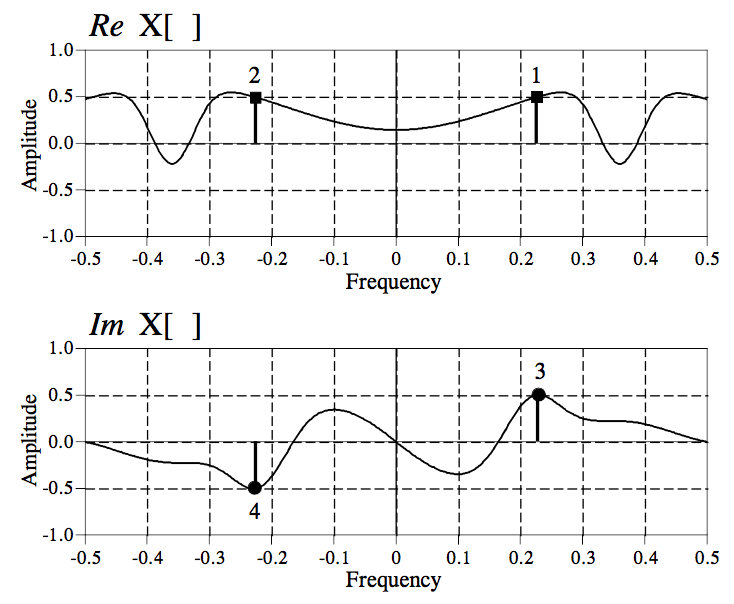
\includegraphics[width=0.7\textwidth]{bilder/dftSymmetrie.png}
 	\caption{Symmetrie des Frequenzbereiches in den Indexen $n = (-N/2 = -0.5*N) ,\ldots ,  (N/2 = 0.5*N)$. Die Marker 1 und 2 haben eine Amplitude von $+0.5$, der Marker 3 hat eine Amplitude von $-0.5$ und Marker 4 eine Amplitude von $+0.5$ }
 	\label{img:symmetrieInDFT}
 \end{figure} 
 
 
Wie zur Einleitung dieses Kapitels erwähnt wurde, wird die Berechnung der komplexen DFT und inversen DFT mit Hilfe eines Algorithmus implementiert, der als \emph{Fast Fourier Transformation} (\textbf{FFT} bzw. \textbf{iFFT}). Die Funktionsweise dieses Algorithmus wird an dieser Stelle aus Platzgründen nicht näher erläutert. Schlussendlich ist das Ergebnis der FFT bzw. iFFT der Frequenz-/Zeit-Bereich nach den in diesen Kapitel vorgestellten definitionen. Die FFT fordert als einzige voraussetzung, dass die Länge des Signals als Potenz von zwei gewählt wird, das heißt Length$(x[\;]) = N = 2^k$. \cite[S. 225 - 226]{dspGuide}

\begin{figure}[h]
	\centering
	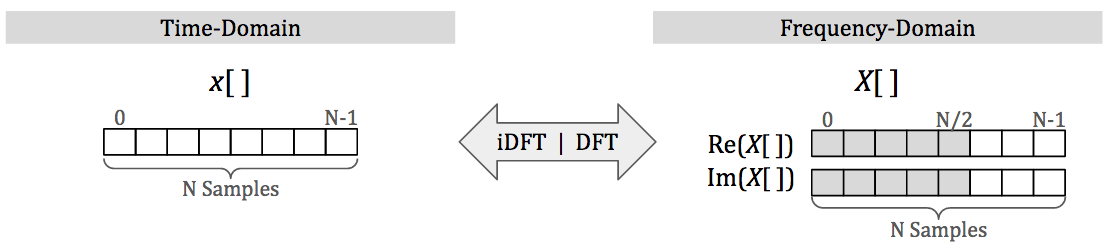
\includegraphics[width=1\textwidth]{bilder/compDFTOverview02.png}
	\caption{Überblick über die komplexe DFT und inverse DFT}
	\label{img:complexDFTOverview}
\end{figure}

\subsection{Short Time Fourier Transform}
\label{sec:stft}

Wie aus Kapitel \ref{sec:comDFT} hervorgeht, enthält die Signal des Zeit-Bereiches die Informationen über den zeitlichen Verlauf des Signals, während der Frequenz-Bereich Aufschluss über Frequenzanteile des Signales gibt. Abbildung \ref{img:stft01} visualisiert den Zusammenhang: Oben ist der Zeit-Bereich eines 1.8 Sekunden langen Signals zu sehen. Es können klar drei nacheinander gespielte Töne erkannt werden. Der Zeit-Bereich macht nicht erkennbar, welche Frequenz-Anteile in den Tönen enthalten sind. Unten ist das Frequenz-Spectrum (Magnituden-Signal im Bereich  $n = 0 ,\ldots, N/2$) abgebildet. Die x-Achse bezeichnet die Frequenz von 0 bis \SI{22050}{\hertz}, die x und die y-Achse werden logarithmisiert dargestellt. Wie zu erkennen ist, gibt das Frequenz-Spectrum einen Eindruck der Frequenz-Anteile des Signals, aber die zeitliche Information über die drei Töne geht verloren.

 \begin{figure}[h]
	\centering
	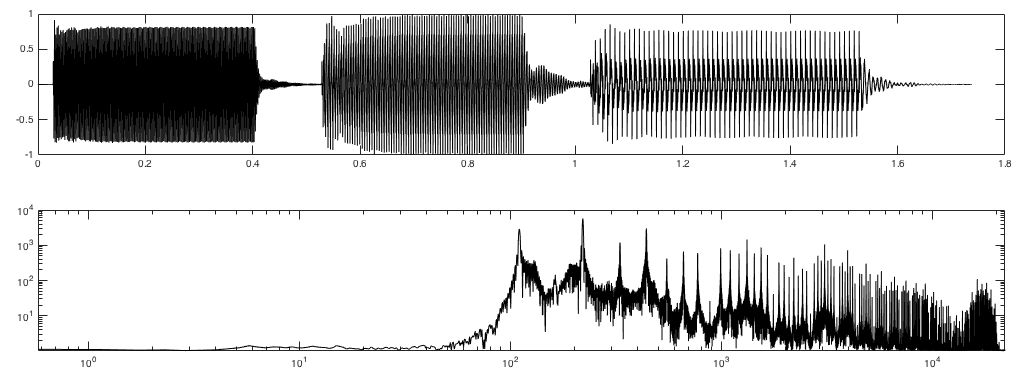
\includegraphics[width=0.8\textwidth]{bilder/stft01.png}
	\caption{Ein 1.8-Sekunden langes Signal. Oben: Der Zeitbereich mit drei klar erkennbaren Events. Unten: Das Frequenz-Spectrum des gesamten Signals mit logarithmisierten Achsen.}
	\label{img:stft01}
\end{figure}

Es ist wünschenswert, einen Kompromiss aus den Vorteilen beider Bereiche zu finden, in dem man das Frequenz-Spectrum kürzerer Zeitabschnitte des Signals bildet. Dazu wird der Zeit-Bereich $x[\;]$ in Fenster der Länge $M$ zerlegt. Die zeitliche Differenz zwischen zwei Fensterns wird als \emph{Hoptime} $R$ bezeichnet. Gleichung definiert die Bildung des Signal-Fensters $x_m[\;]$.\cite{juliusSmith}

 \begin{equation}
x_m[\;] := \quad \mathop{\forall}_{n = 0}^{M-1} :\ x_{m}[n] = x[n+m\cdot R]
\label{eq:signal-Window}
\end{equation}

Abbildung \ref{img:siganlWindows} gibt ein Beispiel für die Zerlegung von $x$ in Signalfenster $x_0[\;] ,\ldots, x_4[\;]$. Die Samplingrate des Signals ist $f_s = 44100$, die Fensterlänge beträgt $M = 22050 / f_s = \SI{0.5}{\second}$ und die Hoptime $R = M / 2= \SI{0.25}{\second}$.

\begin{figure}[h]
	\centering
	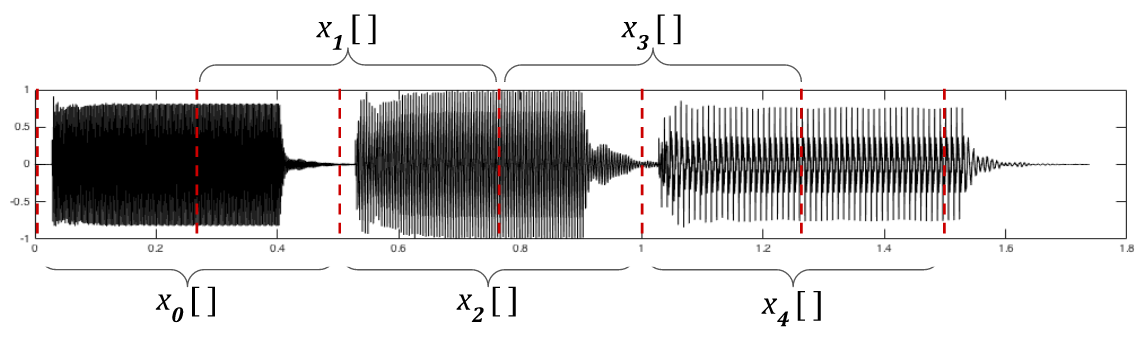
\includegraphics[width=1\textwidth]{bilder/signalWindows02.png}
	\caption{Zerlegung eines Signals in Singal-Fenster}
	\label{img:siganlWindows}
\end{figure}

Als Vorbereitungsschritt für die Transformation der Signal-Fenster in den Frequenz-Bereich wird nun jedes Fenster mit einer sogenannten \emph{Fensterfunktion} (engl \emph{window}) $w[\;]$ multipliziert. Gleichung \ref{eq:hammingWindow} definiert eine der am weitesten verbreiteten Fenster-Funktionen, das \emph{Hamming-Window}. Der Paramter $M$ gibt die länge des Fensters an. Abbildung 	\ref{img:hamming} visualisiert das Hamming-Window. \cite[S. 286]{dspGuide}

 \begin{equation}
w[\;] := \quad \mathop{\forall}_{n = 0}^{M-1} :\ w[n] = 0.54 - 0.46 \cos(\frac{2\pi n}{M} )
\label{eq:hammingWindow}
\end{equation}

 \begin{figure}[h]
	\centering
	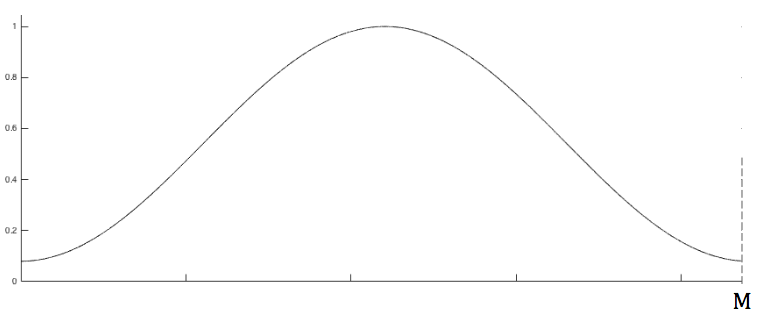
\includegraphics[width=0.4\textwidth]{bilder/hamming01.png}
	\caption{Das Hamming-Window}
	\label{img:hamming}
\end{figure}

Die Gleichung \ref{eq:stft} definiert die \emph{Kurzzeit-Fourier-Transformation} (engl \emph{Short Time Fourier Transformation}, \emph{STFT}), implementiert mit Hilfe der DFT. Dabei wird das Signalfenster $x_m[\;]$ mit der Fensterfunktion $w[\;]$ multipliziert und in das \emph{Frequenz-Fenster} $X_m[\;]$ transformiert.\cite{stft} Abbildung \ref{img:stft02} visualisiert die STFT des Beispiels aus Abbildung \ref{img:siganlWindows}.

 \begin{equation}
\text{STFT}\{x_m[\;]\} = X_m[\;] := \quad \mathop{\forall}_{k = 0}^{M-1} :\ X_m[k] = \sum_{n=0}^{M-1} x_m[n] \cdot w[n] \cdot e^{-i 2\pi k \frac{n}{N}}
\label{eq:stft}
\end{equation}

 \begin{figure}[h]
	\centering
	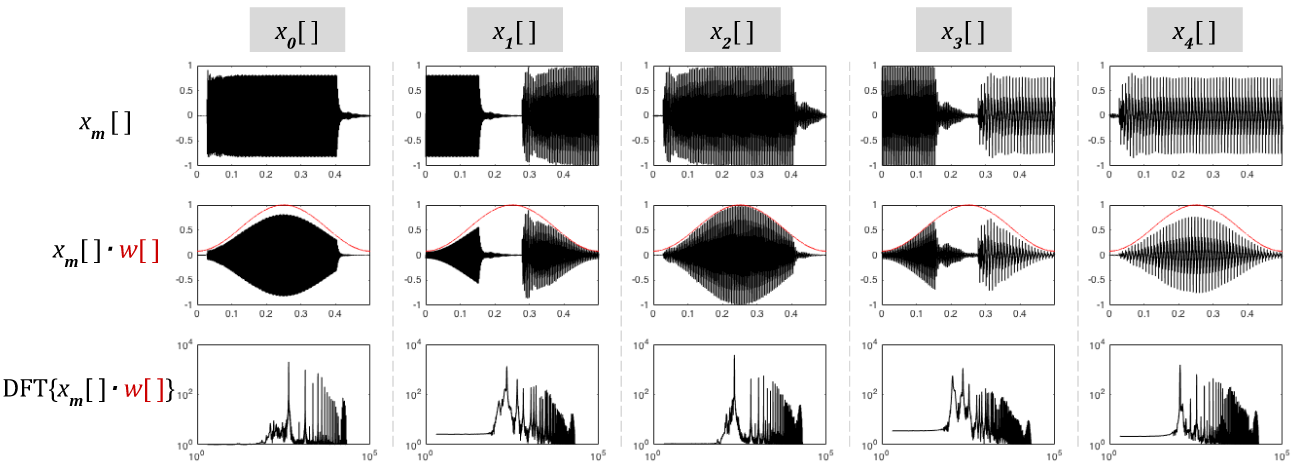
\includegraphics[width=1\textwidth]{bilder/stft03.png}
	\caption{STFT des Beispiel-Signals aus Abbildung \ref{img:siganlWindows}}
	\label{img:stft02}
\end{figure}


\section{Filter}
\label{sec:filter}

Ein \emph{Filter} ist eine Funktion, welches ein Eingangs-Signal $x[\;]$ auf ein Sample eines Ausgangssignals $y[n]$ abbildet. Er wird mit Hilfe des sogenannten \emph{Signal Operators} $T_n{\;}$ notiert, wie Gleichung \ref{eq:SignalOperator} definiert. \cite[\glqq Definition of a Filter\grqq ]{introductionToFilters}

 \begin{equation}
T_n \{ x[\;] \} = y[n]
\label{eq:SignalOperator}
\end{equation}

Auf Basis des \ref{eq:SignalOperator} wird die \emph{Transformation} $T\{ \; \}$ als Operation definiert, welche das Signal $x[\;]$ auf ein Signal $y[\;]$ abbildet, in dem $T_n{\;}$ für meherere n angewandt wird, wie Gleichung \ref{eq:TransformationOperator} definiert. Diese Notation ist bereits bekannt aus den Gleichungen der DFT und iDFT bekannt (Gleichungen \ref{eq:complexDFTpolar}, \ref{eq:complexDFTrectanulgar} und \ref{eq:inverseComplexDFTpolar}). \cite[\glqq Definition of a Filter\grqq ]{introductionToFilters}

 \begin{equation}
T \{ x[\;] \} = y[\;] := \quad \mathop{\forall}_{n = n_1}^{n_2} :\ T_n\{x[\;]\} = y[n]
\label{eq:TransformationOperator}
\end{equation}


Besonders interesant im Zusammenahng mit Audioverarbeitung ist die Klasse der \emph{Lineare, Zeit-Invariante Filter} (engl. \emph{Linear Time-Invariant Filters}, \textbf{LTI}-Filter), notiert mit durch $L_n\{  \}$. Dabei handelt es sich um Filter, die die folgenden drei Eigenschaften erfüllen:

\begin{description}
	\item[Scaling], das heißt, dass eine Skalierung des Input-Signals $x[\;]$ um den Faktor $\alpha$ zur Skalierung des Output-Samples $y[n]$ um den selben Faktor führt, wie Gleichung \ref{eq:scaling} definiert.
	
	 \begin{equation}
	L_n\{ \alpha \cdot x[\;] \} = \alpha \cdot y[n]
	\label{eq:scaling}
	\end{equation}
	
	\item[Super-Position], da heißt, dass das Anwenden des Filters auf die Summmer zweier Signale zum selben Ergebnis führt wie die die isolierte Anwendung des Filters auf die beiden Signale mit nachgelagerter Summation, wie Gleichung \ref{eq:super-position} definiert. \cite[\glqq Linear Filters\grqq ]{introductionToFilters}
	
	 \begin{equation}
	L_n\{ x_1[\;] + x_2[\;] \} = L_n\{ x_1[\;]\}  + L_n\{ x_2[\;]\}
	\label{eq:super-position}
	\end{equation}
	
	\item[Zeit-Invariant], das heißt, dass die Verzögerung des Eingangssingals um einen Faktor $n_0$ zur selben Verzögerung der Ausgangs-Samples führt, wie Gleichung \ref{eq:timeInvariance} definiert.\cite[Filters III, S. 2 - 5 ]{dspMichiganSystems}
	
	 \begin{equation}
		L_{n-n_0}\{ x[\;] \} = y[n-n_0]
	\label{eq:timeInvariance}
	\end{equation}
	
\end{description}

An dieser Stelle werden verschiedene Betrachtungsweisen von Filtern vorgestellt. Jede dieser \emph{Repräsentationen} definiert den Filtern vollständig, bietet jedoch unterschiedliche Betrachtungsweisen des Einflusses des Filters auf das Eingangssignal. \cite[Filters III, S. 1 ]{dspMichiganSystems}

\subsection{Differenzengleichung}
\label{sec:differenzengleichung}

Eine Variante der Beschreibung eines Filters ist mit Hilfe einer \emph{Differenzengleichung} nach Gleichung \ref{eq:FilterDifferenceEquation}. In dieser Arbeit wird ein Linearer Filter, welcher durch eine Differenzen-Gleichung implementiert wird, mit dem Operator $ab_n\{\;\}$ gekennzeichnet. Ein solcher Filter wird vollständig durch die Koeffizienten $a_1 ,\ldots, a_N$ und $b_0 ,\ldots, b_M$  definiert. Ein Filter hat somit $N$ a-Glieder und $M+1$ b-Glieder.  \cite[\glqq Difference Equation\grqq]{introductionToFilters}

 \begin{equation}
\begin{split}
ab_n\{x[\;]\}= y[n] = \overbrace{b_0 x[n] + b_1 x[n-1] + \ldots +b_M x[n-M]}^\text{Feed-Forward} \\
\underbrace{-\ a_1 y[n-1] - \ldots - a_N y[n-N]}_\text{Feed-Back} \\
 = \sum_{i=0}^{M} b_i x[n-i] - \sum_{j=1}^{N} a_j y[n-j]
\end{split}
\label{eq:FilterDifferenceEquation}
\end{equation}

Die Glieder $b_0 ,\ldots, b_M$ sind die Koeffizienten des aktuellen Samples und vergangener Samples des Einganssignals, und werden auch als \emph{Feed-Forward}-Koeffizienten bezeichnet. Die Glieder $a_1 ,\ldots, a_N$ sind die Koeffizienten vergangener Samples der Antwort $y[\;]$. Sie werden daher auch als \emph{Feed-Back}-Koeffizienten oder \emph{rekursive Glieder} bezeichnet. Verwendet ein Filter nur $b$-Glieder und kein $a$-Glied, wird er als \emph{Finite Impulse Response}-Filter (\textbf{FIR}-Filter) bezeichnet. Verwendet ein Filter zumindest ein $a$-Glied, wird er als \emph{Infinite Impulse Response}-Filter (\textbf{IIR}-Filter) bezeichnet.\cite[\glqq Difference Equation\grqq]{introductionToFilters}

 \begin{equation}
\begin{gathered}
\text{FIR} := \quad \forall j = [1,N] :\ a_j = 0 \\
\text{IIR} := \quad \exists j \in [1,N]:  a_j \neq 0
\end{gathered}
\label{eq:FilterDifferenceEquation}
\end{equation}

Die \emph{Ordnung} eines Filters wird definiert als die $\max(M,N)$. \cite[\glqq Filter Order\grqq]{introductionToFilters}.

> Hier folgt ein Beispiel für Filter <.

%% ToDo: Fix Indexes ! Use convention!
\subsection{Faltung}
\label{sec:convolution}

Die \emph{Faltung} (engl. \emph{Convolution}) ist eine der Zentralen Operationen zwischen zwei Signalen, so wie die Addition oder die Mulitplikation. Sie wird mit dem Symbol $*$ notiert. Sie wird notiert mit $x[\;]* h[\;] = y[\;]$. 

Die Faltung basiert auf der sogenannten \emph{Faltungs-Summe}, definiert in Gleichung \ref{eq:convolutionSum}. In diesem Zusammenhang wird $x[\;]$ Eingangs- und $y[\;]$ als Ausgangs-Signal bezeichnet. Je nach Anwendungsfall bekommt $h[\;]$ den Namen \emph{Faltungs-Kernel}, \emph{Filter-Kernel} oder einfach \emph{Kernel}. In dieser Arbeit wird die Faltungs-Summe mit dem Operator $h_n\{\;\}$ definiert. \cite[S. 107-108]{dspGuide}

\begin{equation}
h_n\{x[\;]\} = y[n] = x[n] * h[n] = \sum_{i=1}^{M} h[i] \cdot x[n-i] \quad
\label{eq:convolutionSum}
\end{equation}

Wird die Faltung auf alle Samples des Signal $x[\;]$, wird das Ausgangs-Signal $y[\;]$ im Vergleich zum Eingangs-Signal um die Länge des Faltungskern verlängert, wie Gleichung \ref{eq:convolutionTrans} definiert. $x[\;]$ ist ein Signal mit Support$(x[\;]) = [0,N-1]$ und Length$(x[[\;]) = N$. $h[\;]$ ist ein Signal mit Support$(h[\;]) = [0,M-1]$ und Length$(h[\;]) = M$ und $y[\;]$ ist ein Signal mit Support$(y[\;]) = [0,N+M-2]$ und Length$(y[\;]) = N+M-1$.  um die Länge des Faltungskerns verlängert wird. Abbildung 	\ref{img:convolutionExample} zeigt ein Beispiel für die Faltung.\cite[S. 115-120]{dspGuide}

\begin{equation}
h\{x[\;]\} = x[\;] *  h[\;] =  y[\;] := \quad \mathop{\forall}_{n = 0}^{N+M-2} :\ x[n] * h[n] = y[n]
\label{eq:convolutionTrans}
\end{equation}

\begin{figure}[h]
	\centering
	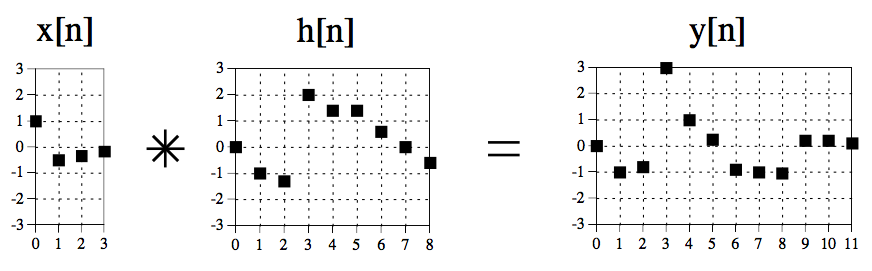
\includegraphics[width=0.7\textwidth]{bilder/convolutionExample.png}
	\caption{Beispiel für die Faltung}
	\label{img:convolutionExample}
\end{figure}

Das neutrale Element der Faltung ist der \emph{Delta-Funktion} $\delta[\;]$, definiert in Gleichung \ref{eq:delta} . Das heißt, dass $x[\;] * \delta[\;] = x[\;]$ . Die Faltung ist kommutativ, das heißt $ x[\;]* h[\;] = h[\;] * x[\;] = y[\;]$ . \cite[S. 107, 113 ]{dspGuide} Weitehrin ist die Faltung assoziativ, das heißt $(x[\;]*y[\;])*z[\;]=x[\;]*(y[\;]*z[\;])$. \cite[S. 133]{dspGuide}

\begin{equation}
\delta [\;] := \quad \mathop{\forall}_{n = -\infty}^{\infty} :\ \delta[n] = 
\begin{cases}
1 \quad , n = 0\\
0 \quad ,  n \neq 0
\label{eq:delta}
\end{cases}
\end{equation}

Die Faltung ist eine der Varianten der Umsetzung von linearen, zeit-invarianten Filtern, neben den in Kapitel \ref{sec:differenzengleichung} vorgestellten Differenzengleichungen. Während ein Filter $L_n\{\;\}]$ in der Repräsentation  als Differenzen-Gleichung vollständig durch die Koeffizienten $a$ und $b$ beschrieben wird, wird bei der Faltungs-Repräsentation ein Filter vollständig durch die Impulsantwort $h[\;]$ beschrieben. Um die Impulsantwort für einen Filter zu erhalten, der zunächst durch einen anderen linearen Filter repräsentiert wird,  filtert man den Delta-Impuls mit diesem Filter, wie Gleichung \ref{eq:howToGetH} definiert. Wird also beispielsweise ein Filter als Differenzengleichung definiert, aber soll mit Hilfe der Faltung umgesetzt werden, so erhält man die Impulsantwort durch $h[n] = ab_n\{\delta[n]\}$.\cite[Impulse-Response Representation ]{introductionToFilters}

\begin{equation}
h[\;] := \quad \mathop{\forall}_{n = 0}^{\infty} :\ h[n] = L_n\{\delta[n]\}
\label{eq:howToGetH}
\end{equation}

Daraus ergibt sich, dass bei FIR-Filtern die Impuls-Antwort endlich ist, das heißt Length$(h[\;]) = M \neq infty$, womit bei einem endlichen Eingangssignal $x[\;]$ auch das Ausgangssignal $y[\;]$ endlich wird. Bei IIR Filtern ist die Impulsantwort hingegen unendlich, da heißt  Length$(h[\;]) = M = infty$, womit auch das Ausngangssignal $y[\;]$ zwangsweise eine unendliche Länge erhält. \cite[\glqq The Finite in FIR\grqq]{introductionToFilters}

\subsection{Multiplikation im Frequenz-Bereich}

Die Faltung im Zeit-Bereich nach den in Kapitel \ref{sec:convolution} vorgestellten Prinzipien entspricht einer Multiplikation im Ortsbereich, wie Formel \ref{eq:fftConvolution} definiert. Das Prinzip wird auch als \emph{FFT-Convolution} bezeichnet. Dazu werden zunächst das Eingangssignal und die Impulsantwort mit Hilfe der DFT in den Frequenz-Bereich transformiert, also $\text{DFT}\{x[\;]\} = X[\;]$ und $\text{DFT}\{h[\;]\} = H[\;]$. Diese beiden Frequenz-Bereiche werden nun miteinander Multipliziert, um den Frequenz-Bereich des Ausganssignals zu erzeugen, das heißt $\forall n = [0,N-1]: X[n] \cdot H[n] = Y[n]$. Mit Hilfe der inversen DFT wird der Frequenz-Bereich in den Zeit-Bereich zurücktransformiert, also $\text{iDFT}\{ Y[\;] \} = y[\;]$. Das so erzeugte Ausgangs-Signal entspricht dem Signal, welches durch die Faltung $x[\;] * h[\;] = y[\;]$ entstanden wäre.\cite[S. 182]{dspGuide}

\begin{equation}
x[\;] * h[\;] = y[\;] = \text{iDFT}\Big\{\ \text{DFT}\{x[\;]\} \cdot \text{DFT}\{h[\;]\}\ \Big\}
\label{eq:fftConvolution}
\end{equation}

In Kapitel \label{sec:convolution} wurde erwähnt, dass sich ein Signal $x[\;]$ durch die Faltung um die Länge der Impulantwort ausdehnt. Daher muss sichergestellt werden, dass das Signal $x[\;]$ vor der Transformation in den Frequenz-Bereich mindestens Length$(h[\;]) = M$ 0-Samples an seinem Ende hat, welche gegebenenalls zuerst angehangen werden müssen. Dadurch wird der Frequenz-Bereich von $x[\;]$ nur dahingehend beeinflusst, dass seine Auflösung erhöht wird. Damit die Frequenz-Bereiche $ X[\;]$ und $H[\;]$ multipliziert werden können, müssen sie die selbe Länge haben. Da die Impulsantwort meistens kürzer als das Eingangssignal ist, müssen ihr vor der DFT meist 0-Samples angehangen werden, um sie auf die selbe länge wie das Eingangsssignal \glqq zu strecken\grqq{}.\cite[S. 183 -184]{dspGuide}

Ein weiterer Vorteil der FFT-Convolution ist, dass Einblick über den Einfluss des Filters auf den Frequenz-Bereich des Eingangs-Signals zur Erzeugung des Ausgangs-Signals gibt. Abbildung \ref{img:convolutionExample} verdeutlicht dieses Prinzip am Beispiel des \glqq windowed Sync Filters\grqq.  Links ist der Zeit-Bereich des Filter-Kernels zu sehen, rechts der Frequenzbereich $\text{DFT}\{h[\;]\} = H[\;]$. Der Frequenz-Bereich macht deutlich dass es sich bei der Impuls-Antwort um einen Tiefpass-Filter handelt, also ein Filter, welcher hohe Frequenzen des Eingangs-signals $x[\;]$ bei seiner Anwendung blockiert, aber tiefe Frequenzen jedoch passieren lässt.\cite[S. 180]{dspGuide}

\begin{figure}[h]
	\centering
	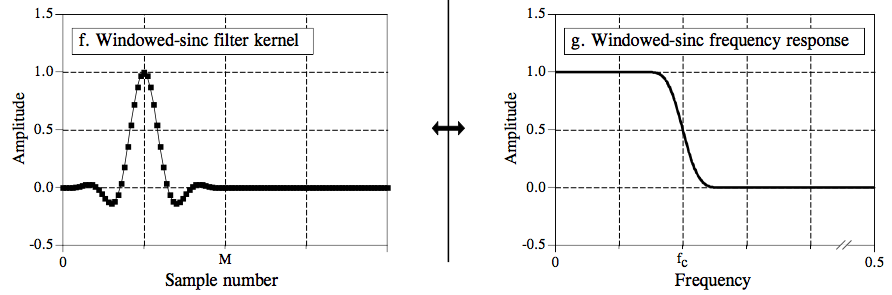
\includegraphics[width=1\textwidth]{bilder/lowPassFilter.png}
	\caption{Links: Zeit-Bereich einer Impulsantwort $h[\;]$ des \glqq windowed Sync Filters\grqq. Rechts: Frequenz-Bereich dieser Impulsantwort $\text{DFT}\{h[\;]\} = H[\;]$ \cite[S. 287]{dspGuide}}
	\label{img:convolutionExample}
\end{figure}

Da ein FIR-Filter eine endlich lange Impulsantwort hat, folgt daraus auch ein endlichlanger Frequenz-Bereich. Ein IIR-Filter hingegen hat einen unenlich lange Impulsantwort und somit auch einen unendlich langen Frequenz-Bereich.

\section{akustische Modellierung der menschlichen Stimme}
\label{sec:theVoice}

An dieser Stelle wird die ein akustisches Modell der menschlichen Stimme vorgestellt. Folgende Organe sind an der Produktion der menschlichen Stimme beteiligt. Abbildung \ref{img:schematicVocalOrgans} visualisiert diese Organe schematisch.

\begin{enumerate}
	\item \textbf{Lunge / Lung}, welcher einen Luftstrom als Grundlage der Lutäußerung erzeugt
	\item \textbf{Stimmbäner / Vocal Chords}, platziert im Kehlkopf (engl. Larynx). Sie erzeugen auf Basis des Luftstroms einen Ton, bezeichnet als \emph{Glottal Source}. Werden die Stimmbänder leicht gespannt, vibrieren sie und erzeugen einen Ton, dass heißt ein im zeit-bereich (quasi-) periodisches Signal (engl. \emph{periodic Source}). Sind die Stimmbänder stark gespannt und nur leicht geöffnet, erzeugen Sie ein Rauschen (engl. \emph{turbulance Source}). Ein durch vibration erzeugter Ton wird als \emph{stimmhaft} bezeichnet, ein durch Rauschen erzeugter Ton als \emph{stimmlos}. Der Ton wür über den Schlund weitergegeben (engl Pharynx) weitergegeben. 
	\item  \textbf{Vokaltrakt / Vocal-Tract}, bestehend aus der Mundhöhle und den Namenraum. Das Velum bestimmt, ob der Ton der Stimmbänder in die Mundhöhle oder den Nasenraum weitergeleitet wird. Je nach Stellung der Zunge, Kiefer, Lippen etc. wird der von den Stimmbändern erzeugte Ton verschieden moduliert. Resonanzen, die durch den Vokaltrakt entstehen, werden als \emph{Formanten} bezeichnet. \cite[S. 62]{cryModel} \cite{speechProduction}
\end{enumerate}
	
\begin{figure}[h]
	\centering
	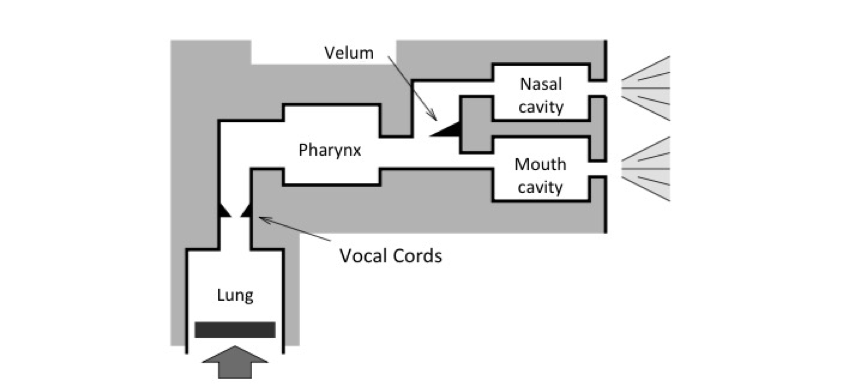
\includegraphics[width=0.5\textwidth]{bilder/SchematicVocalOrgans.png}
	\caption{Schematische Übersicht über die Organe der Spracherzeugung \cite{speechProduction}}
	\label{img:schematicVocalOrgans}
\end{figure}	

Die menschliche Laut-Prudktion wird nach dem so genannten \emph{Source-Filter-Modell} modelliert. Der periodische Ton, der durch die Stimmbänder erzeugt wird, wir angenähert durch einen Impuls-Zug (produziet durch die Stimmbänder), welcher durch den Schlund als linearen Filter leicht wird. Der stimmlose , nicht-periodische Ton wird durch weißes Rauschen angenähert. Der so erzeugte periodische oder nicht-periodische Ton wird als das Eingangs-Signal $u[\;]$ bezeichnet. Dieses Signal wird daraufhin an den Vocaltrakt weitergeben, welcher als linearer, zeitinvarianter Filter mit der Impulsantwort $v[\;]$ angenommen wird. Diese Impulsantwort ist abhängig von der Konfiguraiton der Organe des Vokaltraktes. Die Lippen werden als zweiter linearer, zeit-invarianter Filter mit der Impulsantort $r[\;]$. Das Ausgangssignal $y[\;]$ entsteht also aus der glottal Source $u[\;]$ und den zwei linearen, zeit-invarianten Filtern nach Gleichung \ref{eq:source-Filter-Model}. dargestellt als Faltung im Zeit-Bereich oder Mulitplikation im Frequenz-Bereich.
Abbildung \ref{img:source-filter-model} visualsiert dieses Vorgehen Schematisch. \cite[S. 62 - 63]{cryModel} \cite{speechProduction}

\begin{equation}
\begin{gathered}
u[\;] * v[\;] * r[\;] = y[\;] \\
U[\;] \cdot V[\;] \cdot R[\;] = Y[\;] 
\end{gathered} 
\label{eq:source-Filter-Model}
\end{equation}

\begin{figure}[h]
	\centering
	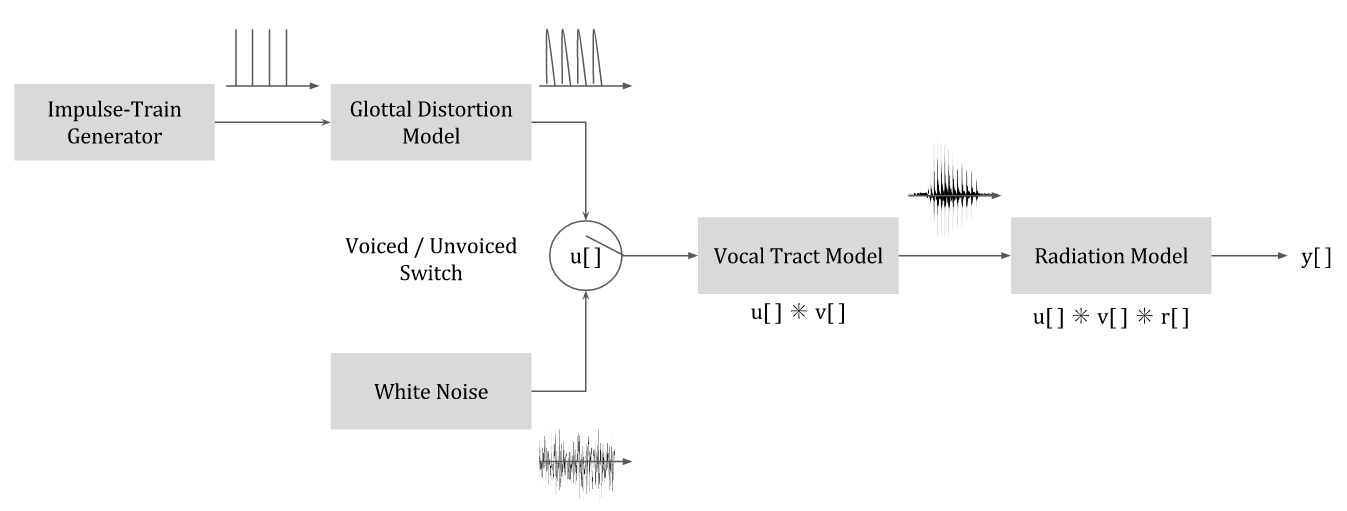
\includegraphics[width=1\textwidth]{bilder/source-filter-model.png}
	\caption{Schematische über das Source-Filter-Model \cite[S. \glqq Source estimation\grqq, S. 17]{ricardo_ceps}}
	\label{img:source-filter-model}
\end{figure}	

Abbidlung \ref{glottalSource} zeigt die Zeitbereiche der periodic und der turbulance Source im Detail. Wie zu sehen ist, bestimmt der zeitliche Abstand zwischen den Impulsen die Grund-Frequenz der Stimme. Dieses Signal $p[\;]$ wird durch die Stimmbändern gefiltert und um den Zeit-Bereich der periodic Source ensteht $G\{p[\;]\} = u_p[\;]$. Darunter ist der Zeit-Bereich des weißen Rauschen zu sehen. \cite[Source]{speechAcoustics}

\begin{figure}[h]
	\centering
	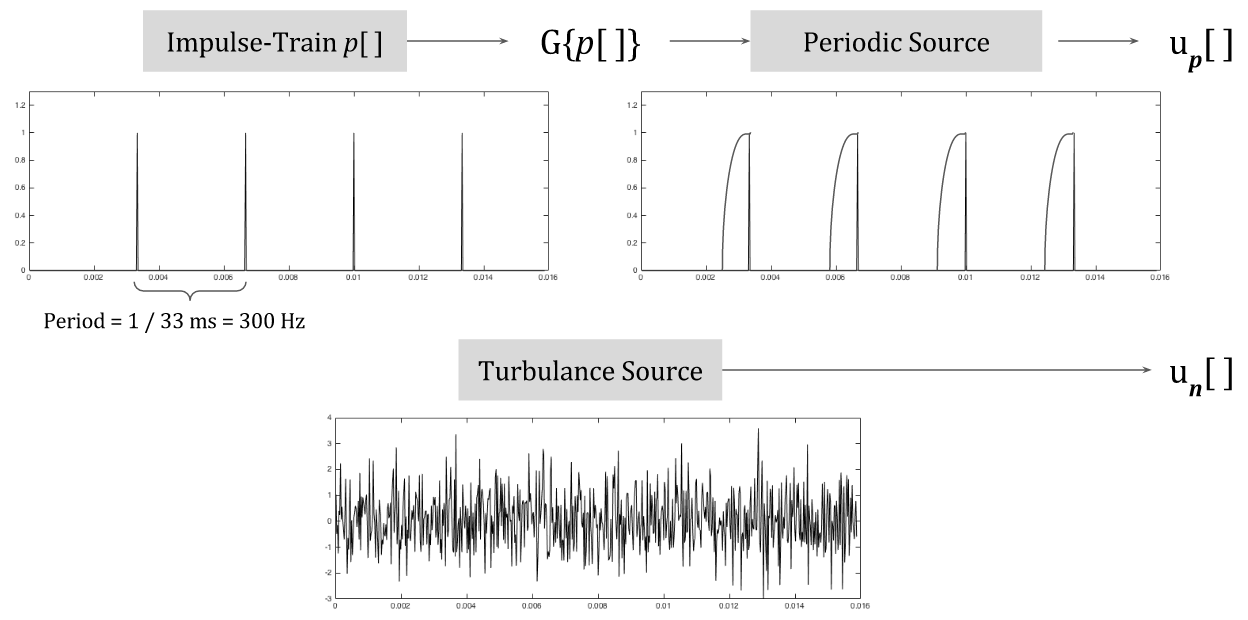
\includegraphics[width=0.8\textwidth]{bilder/glottalSource.png}
	\caption{Zeit-Bereiche der periodic und der turbulance Source \cite[Source]{speechAcoustics}}
	\label{img:glottalSource}
\end{figure}	

Abbildung \ref{img:sourceFilerSpectra} zeigt die Betrachtung der Frequenz-Bereiche des Source-Filter-Modells. Die periodic Source ($U[\;]$ links) zeichnet sich im Frequenz-Bereich durch gleichmäßig verteilte Spitzen aus, die mit steigender Frequenz an Amplitude verlieren. Jeweils zwei Spitzen haben einen Abstand von $f$ zueinander, also in diesem Fall $\SI{300}{\hertz}$. Die Frequenz-Antwort des Vocal Tract Model $V[\;]$ zeichnet sich durch Resonanz-Frequenzen aus, in diesem Beispiel sind 4 erkennbar. Das Radiation Model $R[\;]$ wird als Hochpass-Filter angenähert, also ein Filter, welcher hohe Frequenzen passieren lässt und tiefe blockiert. Das Ausgangssignal $U[\;] \cdot V[\;] \cdot R[\;] = Y[\;] $ zeigt den Einfluss der Filter auf das Eingangssignal.\cite[Source estimation]{ricardo_ceps}, \cite[Vocal Tract Resonance]{speechAcoustics}

\begin{figure}[h]
	\centering
	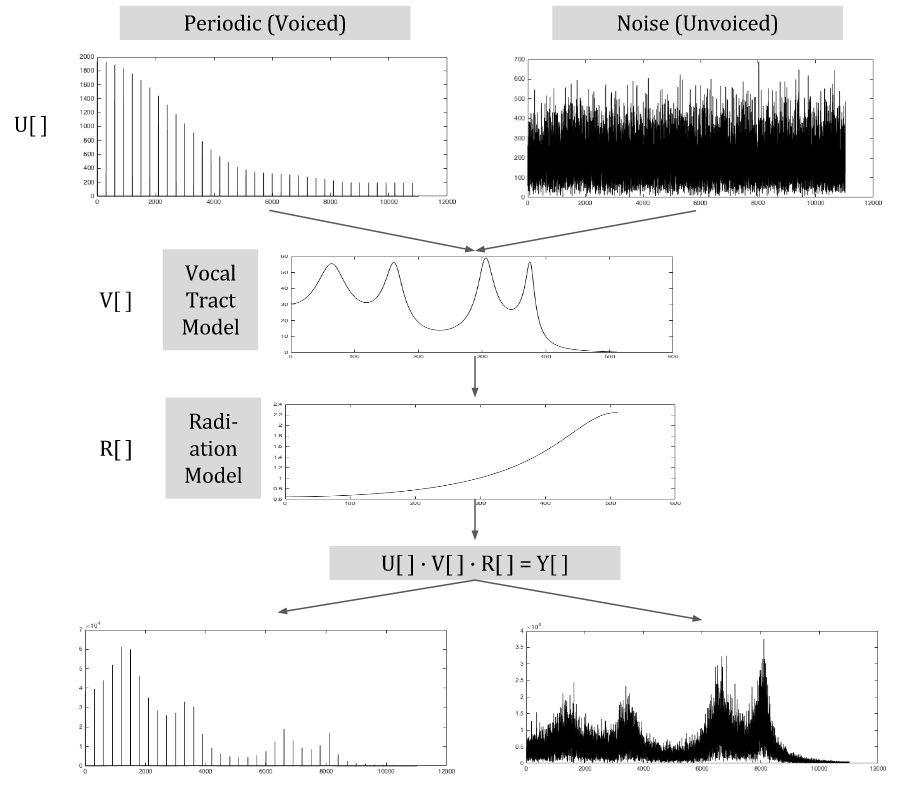
\includegraphics[width=1\textwidth]{bilder/sourceFilterSpectra.png}
	\caption{Betrachtung der Frequenz-Bereiche des Source-Filer-Modell }
	\label{img:sourceFilerSpectra}
\end{figure}	

Abbildung \ref{img:pitchPeaks} zeigt anhand des Frequenz-Spectrums eines stimmhaften Sprachsignals, wie die die Grundfrequenz und die harmonischen Obertonwellen erkannt werden: Die Grundfrequenz $N_0$ ist Bezüglich des Zeit-Bereiches nach Formel \ref{eq:periodicity} definiert. Im Frequenz-Bereich sind die Grund-Frequenz und die harmonischen Oberwellen als die \glqq vielen, kurzen Spitzen\grqq{} erkennbar. Die Frequenz der ersten dieser Spitzen entspricht der Grund-Frequenz $N_0$, in diesem Beispiel $\SI{250.7}{\hertz}$. Die harmonsichen Oberwellen entsprechen dem doppelten, dreifachen, \ldots dieser Grundfrequenz und werden bezeichnet hals $H_1, H_2, \ldots$. Die Grundfrequenz ist \emph{nicht zwingend} die Spitze der höchsten Amplitude! Durch den Einfluss des Vokaltrackts als Filter können harmonische Oberwellen eine höhere Amplitude als die Grundfrequenz haben. Vielmehr lässt sich durch den kleinsten gemeinsamen Teiler der Frequenzspitzen auf die Grundfrequenz schließen.\cite[S. 52 - 53]{sprachverarbeitung}

\begin{figure}[h]
	\centering
	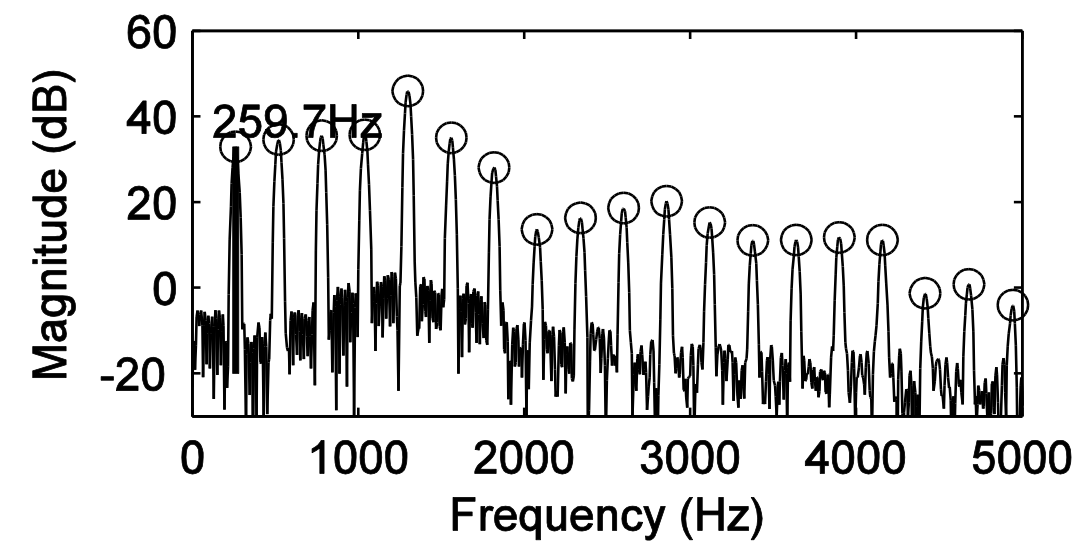
\includegraphics[width=0.5\textwidth]{bilder/pitchPeaks.png}
	\caption{ Grundfrequenz und Harmonische Oberwellen eines Sprachsignals.}
	\label{img:pitchPeaks}
\end{figure}	

Abbildung \ref{img:formants} \footnote{Bildquelle: \url{http://hyperphysics.phy-astr.gsu.edu/hbase/index.html}} verdeutlicht, wie das als linearer, Zeit-Invarianter Filter modellierte Vokaltrakt mit Hilfe von Formanten beschrieben wird. Die Formanten spielen vor allem bei der Beschreibung von Vokalen eine Rolle. Formanten sind lokale Maxima im Spektrum, die dadurch erzeugt werden, dass der Vokaltrakt Resonanzfrequenzen erzeugt. Die Formanten werden von links nach rechts durchnummeriert, von $F_1 ,\ldots\,F_n$. Jeder Formant wird durch seine Mittenfrequenz, seine Bandbreite und seine Amplitude beschrieben, das wichtigste Merkmal ist jedoch die Mittenfrequenz. Mit steigender Frequenz nimmt die Amplitude der Formanten ab, der dominanteste Formant ist also immer der erste. Daher werden meist nur die ersten 2 oder 3 Formanten zur Beschreibung eines Vokals verzeichnet. Für verschiedene Sprachen sind allerlei Tabellen zu finden, welche die Formantenfrequenzen der Vokale listen.\cite[S. 19]{sprachverarbeitung}

\begin{figure}[h]
	\centering
	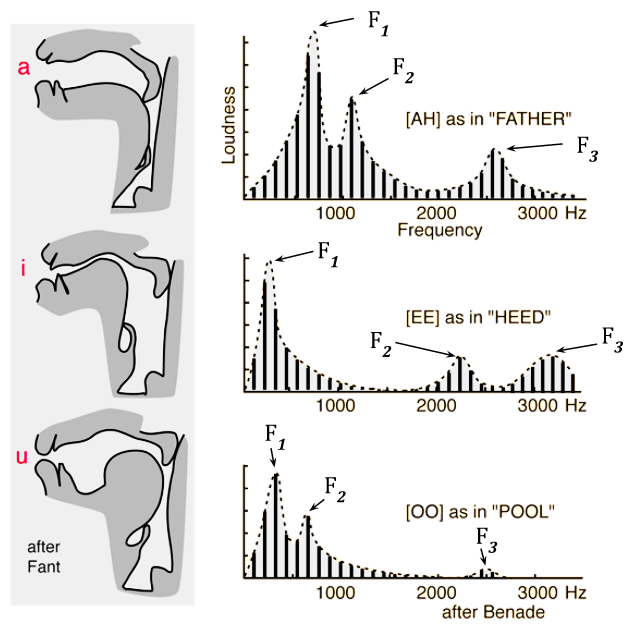
\includegraphics[width=0.7\textwidth]{bilder/formants02.png}
	\caption{Formanten im Sprach-Signal}
	\label{img:formants}
\end{figure}	

Da Sprache etwas zeitlich dynamisches ist, befinden sich sowohl die Glottal Source als auch der Filter des Vokaltraktes und der Lippen in ständiger Veränderung. Da die Informationen der Sprache vor allem im Frequenz-Bereich codiert sind, wird die in Kapitel \ref{sec:stft} vorgstellte Short Time Fourier Transformation für die Visualisierung von Sprache eingesetzt. Dabei wird auf der x-Achse die Zeitpunkte der Fenster, auf der y-Achse die Frequenz dargestellt. Die Frequenz-Fenster werden sozusagen \glqq auf die Seite gelegt\grqq{}, damit ihr zeitlicher Verlauf übersichtlich betrachtet werden kann. Die Amplitude der entsprechenden Frequenz wird farblich oder durch Helligkeiten codiert, abhängig von der konkreten Implementierung des Spectograms. Je länger das Zeitfenster der STFT, desto besser die Auflösung bezüglich des Frequenz-Bereiches, desto schlechter ist jedoch  die zeitliche Auflösung. Je kürzer die Zeitfenster der STFT, desto besser wird der zeitliche Verlauf bei sinkender Frequenz-Auflösung erkennbar.\cite[S. 48 - 50]{sprachverarbeitung} \cite[Acoustic Representations of Speech]{speechAcoustics}. Abbildung \ref{img:formants} zeigt ein Beispiel für zwei Spectogramme mit unterschiedlichen Fenstergrößen der STFT, angewandt auf einem 9 sekunden langen Signal mit Baby-Weinen. Es ist zu erkennen, wie bei sinkender Fensterlänge der zeitliche Verlauf besser erkennbar, jedoch die einzelnen harmonsichen Obertöne weniger gut voneinander unterscheidbar sind. Inbesondere bei der Analyse von Audiosignalen des Weinens der Neugeborenen von Golub und Corwin waren \cite{cryModel} waren Auswertungen von Spectogrammen von Zentraler Bedeutung.
%%Citation from Cry as a Signal!!

\begin{figure}[h]
	\centering
	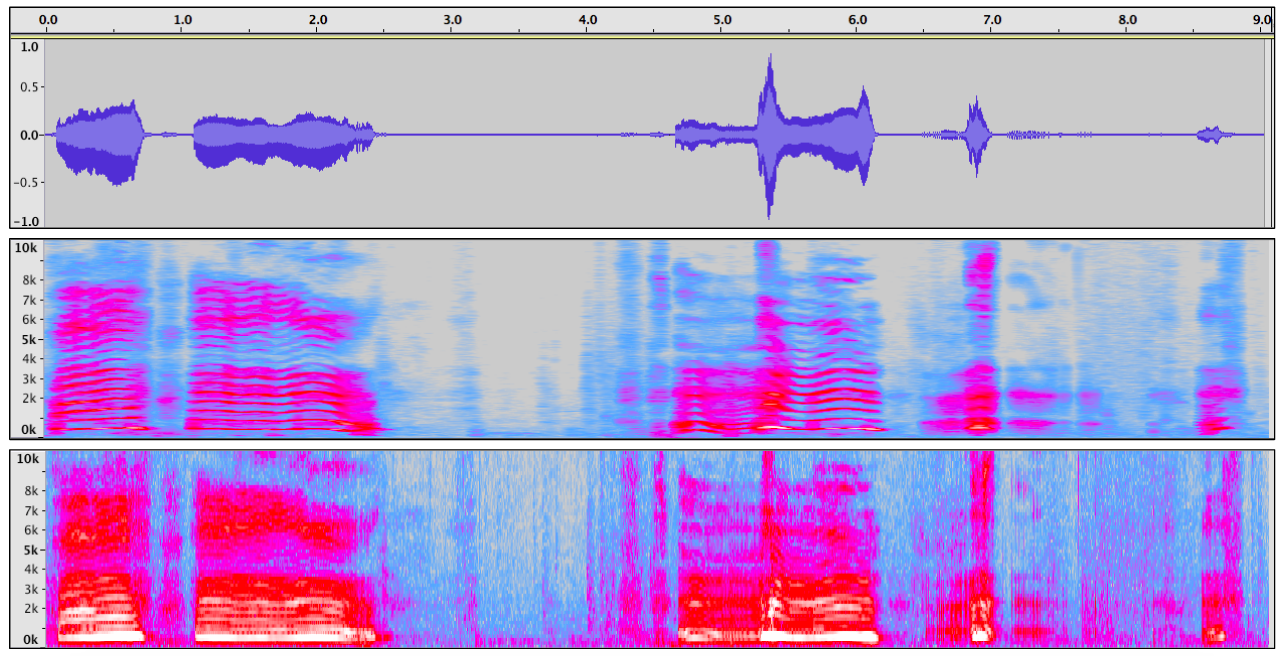
\includegraphics[width=0.7\textwidth]{bilder/spectogram03.png}
	\caption{Spectogram von Baby-Weinen. Rot = Hohe Amplituden, Blau = niedrige Amplituden. Oben: Zeit-Bereich. Mitte: Spectogram mit einer Fensterlänge von $\SI{185}{\milli\second}$(8192-Sample DFT). Unten: Spectogram mit einer Fensterlänge von $\SI{5}{\milli\second}$} (265-Sample DFT).
	\label{img:formants}
\end{figure}	


\section{Feststellung von Periodizität in Signalen}

Die Feststellung von Periodizität in Zeit-Bereich in einem Signal hat eine besondere Rolle in der Sprachverarbeitung. Ein Ensatzgebiet, welches in dieser Arbeit weiter von Bedeutung sein wird, ist die Voice-Activity-Detection, die Feststellung des Vorhandenseins von Stimme in einem Signal. \cite{vad_Lisboa} Ein weiteres Einsatzgebiet ist die Tonhöhenerkennung. \cite{pitch-paper-overview}  \cite[S. 1 - 2]{pitchHistory}

Ein Sprachsignal ist 1.) nur über kurze Zeitfenster periodisch, da sich die Tonhöhe jederzeit ändern kann, und 2.) selbst bei \glqq perfekt gewählter Fensterlänge\grqq{} nicht perfekt periodisch, sondern nur annhäernd periodisch (\emph{quasi periodisch}).\cite[S. 1 - 2]{pitchHistory} Formel \ref{eq:quasi-periodicity} definiert diese Aussage als Formel für den Zeit-Bereich.

\begin{equation}
 x[n+N] \approx x[n]
\label{eq:quasi-periodicity}
\end{equation}

%Kapitel einfügen >.<
Über die Jahre wurde eine Vielzahl an Methoden zur Feststellung der Periodizität entwickelt. An dieser Stelle wird eine Auswahl vorgestellt, die für die Voice-Activity-Deteciton in Kapitel xxx von Bedeutung sind.

%\subsection{Zero-Crossing-Rate}

%Bei der Zero-Crossing-Rate (ZCR) wird gezählt, wie oft das signal die x-Achse überschreitet, also das  Vorzeiche wechselt Formel \ref{eq:zcr} definiert die ZCR.\cite[S. 335]{vad_ceps}

%\begin{equation}
%\text{ZCR}(x_m[\;]) = \sum_{n=n_1}^{n_2} | \text{sgn}(x_m[n]) -  \text{sgn}(x_m[n-1]) |
%\label{eq:zcr}
%\end{equation}

%Mit Hilfe der Zer-Crossing-Rate wird nicht Periodizität, sondern das Nicht-Vorhandensein von Rauschen nachgewiesen. Da Rauschen eine höhere Zero-Crossing-Rate hat als ein periodisches Signal (mit einer Grundfrequenz im Bereich der menschlichen Stimme), sprechen niedrige Zero-Crossing-Rates für das vorhandensein von Periodizität. Der Nachteil dieser Methode ist, dass bei kompletter Abwesenheit von Hintergrundrauschen eine ZCR von 0 fälschlicherweise für Periodzittät sprechen würde. \cite[S. 335]{vad_ceps}

%\subsection{Most Dominant Frequenzcy}

%Die dominansteste Frequenz (Most Dominant Frequency) wird nach Formel \ref{eq:domFreq} als die Frequenz mit der höchsten Amplitude des Frequenz-Fensters $(X_m[\;]$ definiert. \cite[S. 2550]{vad_Easy} 

%\begin{equation}
%f_{Dom}(X_m[\;]) = \argmax_f\{X_m[f]\}
%\label{eq:domFreq}
%\end{equation}
 
 %Wie Abbdilung in\ref{img:source-filter-model} und \ref{img:pitchPeaks} zu sehen ist, hat der Fequenz-Bereich eines periodisches Signals die dominanteste Frequenz im Bereich der Grund-Frequenz-Frequenz oder einer harmonischen Oberwelle, während Rauschen die Dominanteste Ferquenz an einer beliebigen Position haben kann. Nach Moattar und Homayounpour \cite[S. 2550]{vad_Easy} ist die dominanteste Frequenz bei Rauschen tiefer zu erwarten als bei einem periodischen Signal. 

\subsection{Autokorrelation}

Die Korrelation wurde in Kapitel \ref{sec:correlation} vorgestellt. Bei der Autokorrelation wird ein Signal mit einer vezögerten Variante von sich selber korrelliert. Gleichung \ref{eq:ACorr} definiert die Autokorrelation des Signals eines $N$-Samples langen Signals $x[\;]$ mit einer um das Lag $k$ verzögerten Variante von sich selber.

\begin{equation}
\text{A-Corr}_k(x[\;]) = \sum_{n=k}^{N} x[n-k] \cdot x[n]
\label{eq:ACorr}
\end{equation}

Wie bei der in Kapitel \ref{sec:correlation} vorgestellten Cross-Correlation gibt es verschiedene Möglichkeiten der Normalisierung der Korrelationswertes in Bezug auf die Signalenergien. Gleichung \ref{eq:NACorr} definiert die normalisierte Autokorrelation.\cite{vad_Lisboa}

\begin{equation}
\text{NA-Corr}_k(x[\;]) = \frac{\sum_{n=k}^{N} x[n-k] \cdot x[n]}{ \sqrt{\sum_{n=1}^{N-k}  x[n]^2}  \cdot  \sqrt{\sum_{n=k}^{N}  x[n]^2} }
\label{eq:NACorr}
\end{equation}

Nun wird das Autokorrelations-Signal $a[\;]$ erstellt, in dem Gleichung \ref{eq:ACorr} oder \ref{eq:NACorr} für verschiedene $k = k_min \ldots k_max$ angewandt wird, wie Gleichung \ref{eq:a-Signal} definiert. 

\begin{equation}
a[\;] := \quad \mathop{\forall}_{k = k_{min}}^{k_{max}} :\ a[k] = \text{NA-Corr}_k(x[\;]) 
\label{eq:a-Signal}
\end{equation}

Ein hoher Wert des Signals $a[\;]$ an der Position $k$ spricht für eine Periodizität des Signals mit der Frequenz $f =  f_s / k $. Es ist üblich, den Bereich $[k_{min},k_{max}]$ so einzuschränken, dass die Autokorrelation nur für den Frequenz-Raum durchegeführt wird, in dem man Periodizität erwartet. 

\begin{figure}[h!]
	\centering
	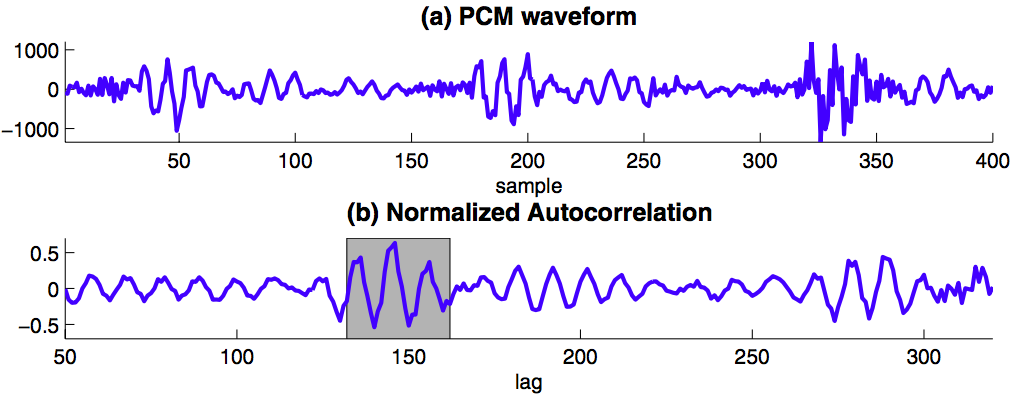
\includegraphics[width=0.8\textwidth]{bilder/acorr.png}
	\caption{Autokorrelation eines Signals}
	\label{img:acorr}
\end{figure}	

Abbildung \ref{img:acorr} verdeutlicht das Vorgehen an einem Beispiel. Gezeigt wird  in (a) der Zeit-Bereich eines quasi-periodischen Signals $x[\;]$, welches mit einer Sampling-Frequenz von $f_s = \SI{16.000}{\hertz}$ aufgenommen wurde. Es wird eine Periodizität im Bereich $\SI{50}{\hertz} - \SI{400}{\hertz}$ vermutet, daher wird die normalisierte Autokorrelation nach Formel \ref{eq:a-Signal} durchgeführt mit den Lags $k_{min} = \SI{16.000}{\hertz} / \SI{400}{\hertz} = 40$ bis $k_{max} = \SI{16.000}{\hertz} / \SI{50}{\hertz} = 320$. (b) zeigt das so entstandene Signal $a[\;]$. Das Maximum an der Stelle $k = 146$ weisst auf eine Grundfrequenz von $N_0 \approx \SI{109}{\hertz}$ hin. Dabei kann es sich jedoch auch um die Frequenz einer Harmonische Schwingung handeln, welche durch den Einfluss des Filters des Vokaltraktes verstärkt wurde. Es kann sich auch um die Hälfte der Grundfrequenz handeln, da wie in Kapitel \ref{sec:signalFoundations} erläutert, ein Signal mit der Periode $N$ ebenfalls eine Periodizität bezüglich $2N, 3N,\ldots$ aufweist. \cite{vad_Lisboa} \cite[S. 24]{dspMichigan}

\subsection{Cepstrum}

Das Cepstrum wird nach Gleichung \ref{eq:cepstrum} als die inverse DFT des Logarithmus des Magnitudensignals des Frequenz-Bereiches definiert. 

\begin{equation}
ceps[\;] =  \text{iDFT}\Big\{ \log \Big(\ \big|\ \text{DFT}\{x[\;]\} \big|\ \Big) \Big\}
\label{eq:cepstrum}
\end{equation}

\begin{figure}[h]
	\centering
	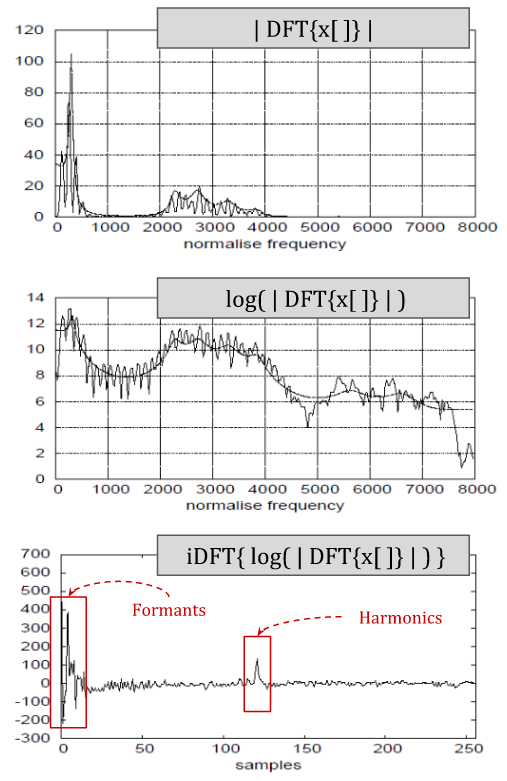
\includegraphics[width=0.6\textwidth]{bilder/cepstrum04.png}
	\caption{Berechnung des Cepstrums}
	\label{img:cepstrumOverview}
\end{figure}	


Das Vorgehen wird mit Hilfe des Beispiels aus Abbildung \ref{img:cepstrumOverview} erläutert. $ |\ \text{DFT}\{x[\;]\} \big| $  zeigt das Spectrum (Magnituden-Signal) eines \glqq typischen stimmhaften\grqq{} Signals $x[\;]$. Es sind die in Kapitel \ref{sec:theVoice} erläuterten harmonischen Obertöne zu sehen, welche mit steigender Frequenz an Amplitude verlieren. Durch das logarithmieren des Spectrums $\log \Big(\ \big|\ \text{DFT}\{x[\;]\} \big|\ \Big)$ wird die Dynamic des Frequenz-Bereiches verringert und somit der Amplituden-Verlust der höheren Obertöne verringert. Nun stellt man sich vor, dieses Spectrum wäre ein Signal des Zeit-Bereiches. Dieses Signal würde man als ein Quasi-Periodisches Signal mit einer Amplituden-Modulation interpretieren, das heißt ein Signal mit hoher Frequenz, addiert mit einem Signal mit nierdiger Frequenz. Um diese beiden Komponenten voneinander zu trennen, würde man wieder die DFT anwenden, um das Spectrum zu bilden. Diese DFT kommt in dem Fall einer inversen DFT gleichkommt, da das Magnituden-Signal verworfen wird. Man erwartet in diesem \glqq Spectrum vom Spectrum\grqq{} einen Peak im \glqq oberen Frequenz-Bereich\grqq , bedingt durch die harmonischen Oberwellen, sowie einen Peak im  \glqq unteren Frequenz-Bereich\grqq, bedingt durch die Formanten.\cite[Cepstral analysis]{ricardo_ceps}

Der Bereich dieser \glqq Fouriertransformation der Foueriertransformation\grqq{} wird als \emph{Cepstrum} bezeichnet. Cepstrum ist ein ein Wortspiel, welches durch die Umkehrung der ersten vier Buchstaben des Wortes "Spectrum" ensteht. Die Unabhängige Variable des Cepstrum folgt dem Wortspiel und wird als \emph{Quefrency} bezeichnet. Damit wird verdeutlicht, dass die unabhängige Variable des Cepstrum zwar mathematisch betrachtet die Zeit darstellt, jedoch als Frequenz interpretiert wird.\cite[S. 7]{ricardo_ceps}

\begin{figure}[h]
	\centering
	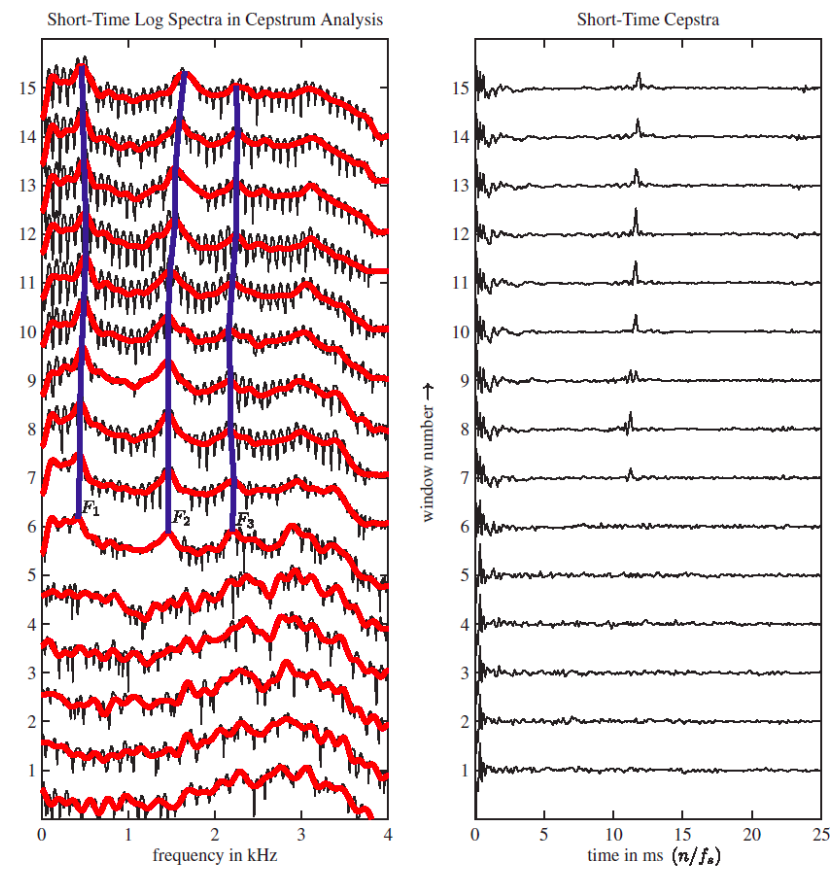
\includegraphics[width=0.6\textwidth]{bilder/cepstrum05.png}
	\caption{Aufkommen eines Peaks im oberen Quefrency-Bereich bei stimmhaften Signalfenstern \cite[S. 17]{ricardo_ceps}}
	\label{img:cepstrumVoicedPeak}
\end{figure}	

Insbesondere ein Auftauchen eines Peakes im oberen Quefrency-Bereich $> \SI{3}{\milli\second}$ spricht für das vorhandensein von harmonischen Obertönen und somit für periodizität im Signal, wie sie durch Stimme entsteht. Abbildung \ref{img:cepstrumVoicedPeak} verdeutlicht das Prinzip an einem Beispiel. Zu sehen ist die STFT eines Signals mit einer Fensterlänge von $\SI{50}{\milli\second}$ und einer Hopsize von $\SI{12.5}{\milli\second}$. Links wird das Logarithmisierte Spektrum abgebildet, und rechts das Cepstrum. Die Frames 1-5 sind stimmlos, die Frames 8-15 sind stimmhaft, und die zwischen-Frames eine Mischung. Man sieht das Aufkommen eines Peaks bei einer Quefrency $q = \SI{12}{\milli\second}$.\cite[S. 16]{ricardo_ceps}

Abbildung \ref{img:cepstrumPitch} verdeutlicht, wie eine Grundfrequenz $f_0$ im Zeit-Bereich einen Peak im Cepstrum erzeugt. So weist ein Peak an bei der Quefrency $q$ auf eine Grundfrequenz von  $q = f_s/f_0$ hin. Dabei kann es sich, wie bei der Autokorrelation, um einen Oktaven-Fehler handeln, das heißt, dass der höchste Peak das Doppelte oder die Hälfte der eigentlichen Grundrequenz beträgt. \cite{cepstrumPitchTranslation}

\begin{figure}[h]
	\centering
	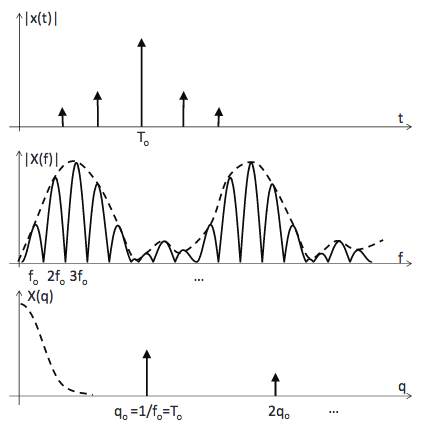
\includegraphics[width=0.6\textwidth]{bilder/cepstrumPitch.png}
	\caption{Feststellung der Grundfrequenz aus dem Cepstrum\cite{cepstrumPitchTranslation}}
	\label{img:cepstrumPitch}
\end{figure}	
